% Qlassifier paper v1.
% Build: tectonic docs/paper/main.tex   (or pdflatex + bibtex; ASCII source, no shell escape)
% Every number comes from docs/paper/generated/ (python scripts/paper_tables.py), which reads the saved results in
% benchmarks/ (see its README.md) and the research runs in experiments/.
\documentclass[aps,pra,reprint,superscriptaddress,nofootinbib,longbibliography]{revtex4-2}

\usepackage{graphicx}
\usepackage{booktabs}
\usepackage{amsmath,amssymb}
\usepackage{xcolor}
\usepackage[colorlinks=true,linkcolor=blue!50!black,citecolor=blue!50!black,urlcolor=blue!50!black]{hyperref}

\graphicspath{{figures/}}

% \val{<key>}: a number written by scripts/paper_tables.py. An unknown key stops the build.
\makeatletter
\newcommand{\qlvalue}[2]{\expandafter\def\csname qlv@#1\endcsname{#2}}
\newcommand{\val}[1]{\ifcsname qlv@#1\endcsname\csname qlv@#1\endcsname\else
  \PackageError{qlassifier}{No value '#1'}{Run python scripts/paper_tables.py}\fi}
\makeatother
% Generated by scripts/paper_tables.py from the saved results. Do not edit: rerun the script.
% Usage in main.tex: \val{key}.
\qlvalue{bc.rows}{569}
\qlvalue{bc.features}{30}
\qlvalue{bc.positives}{212}
\qlvalue{bc.ntrain}{398}
\qlvalue{bc.ntest}{171}
\qlvalue{bc.seeds}{10}
\qlvalue{bc.ratio}{0.430}
\qlvalue{bc.ba}{0.948}
\qlvalue{bc.ba.sd}{0.012}
\qlvalue{bc.ba.ci}{[0.928, 0.968]}
\qlvalue{bc.acc}{0.956}
\qlvalue{bc.auc}{0.991}
\qlvalue{bc.rank}{6th of 12}
\qlvalue{bc.tied}{yes}
\qlvalue{bc.zz.ba}{0.571}
\qlvalue{bc.zz.acc}{0.677}
\qlvalue{bc.trivial.acc}{0.626}
\qlvalue{bc.vszz}{+37.6}
\qlvalue{bc.vszz.ci}{[+34.6, +40.7]}
\qlvalue{bc.vszz.wins}{10/10}
\qlvalue{bc.vszz.acc}{+27.9}
\qlvalue{bc.best}{MLP}
\qlvalue{bc.best.ba}{0.961}
\qlvalue{bc.vsbest}{$-$1.3}
\qlvalue{bc.vsbest.ci}{[$-$3.1, +0.5]}
\qlvalue{bc.vsbest.wins}{0/10}
\qlvalue{bc.vsbest.p}{0.13}
\qlvalue{bc.vsbest.word}{a statistical tie (the CI contains 0)}
\qlvalue{bc.models}{12}
\qlvalue{bc.pub}{0.968}
\qlvalue{bc.pub.method}{QKT}
\qlvalue{bc.vspub}{$-$2.0}
\qlvalue{bc.time.tune}{0.38}
\qlvalue{bc.time.fit}{0.016}
\qlvalue{bc.time.predict}{0.0022}
\qlvalue{bc.noise.shots}{$-$0.12}
\qlvalue{bc.noise.shots.worst}{+0.58}
\qlvalue{bc.noise.shots.r}{0.9984}
\qlvalue{bc.noise.torino}{+0.12}
\qlvalue{bc.noise.torino.worst}{+0.58}
\qlvalue{bc.noise.torino.r}{0.9983}
\qlvalue{bc.noise.fez}{+0.12}
\qlvalue{bc.noise.fez.worst}{+0.58}
\qlvalue{bc.noise.fez.r}{0.9983}
\qlvalue{bc.noise.brisbane}{+0.12}
\qlvalue{bc.noise.brisbane.worst}{+0.58}
\qlvalue{bc.noise.brisbane.r}{0.9983}
\qlvalue{bc.noise.max}{+0.12}
\qlvalue{bc.qubits}{4}
\qlvalue{bc.twoq}{0}
\qlvalue{bc.depth}{6}
\qlvalue{bc.circuits}{1,707}
\qlvalue{bc.circuitratio}{1,420}
\qlvalue{iono.rows}{351}
\qlvalue{iono.features}{33}
\qlvalue{iono.positives}{126}
\qlvalue{iono.ntrain}{245}
\qlvalue{iono.ntest}{106}
\qlvalue{iono.seeds}{10}
\qlvalue{iono.ratio}{0.433}
\qlvalue{iono.ba}{0.925}
\qlvalue{iono.ba.sd}{0.018}
\qlvalue{iono.ba.ci}{[0.894, 0.955]}
\qlvalue{iono.acc}{0.934}
\qlvalue{iono.auc}{0.969}
\qlvalue{iono.rank}{2nd of 12}
\qlvalue{iono.tied}{yes}
\qlvalue{iono.zz.ba}{0.698}
\qlvalue{iono.zz.acc}{0.772}
\qlvalue{iono.trivial.acc}{0.642}
\qlvalue{iono.vszz}{+22.6}
\qlvalue{iono.vszz.ci}{[+13.9, +31.4]}
\qlvalue{iono.vszz.wins}{10/10}
\qlvalue{iono.vszz.acc}{+16.2}
\qlvalue{iono.best}{RBF-SVM}
\qlvalue{iono.best.ba}{0.926}
\qlvalue{iono.vsbest}{$-$0.2}
\qlvalue{iono.vsbest.ci}{[$-$3.1, +2.7]}
\qlvalue{iono.vsbest.wins}{5/10}
\qlvalue{iono.vsbest.p}{0.89}
\qlvalue{iono.vsbest.word}{a statistical tie (the CI contains 0)}
\qlvalue{iono.models}{12}
\qlvalue{iono.pub}{0.911}
\qlvalue{iono.pub.method}{QKT}
\qlvalue{iono.vspub}{+1.4}
\qlvalue{iono.time.tune}{0.29}
\qlvalue{iono.time.fit}{0.009}
\qlvalue{iono.time.predict}{0.0014}
\qlvalue{iono.noise.shots}{$-$0.19}
\qlvalue{iono.noise.shots.worst}{0.00}
\qlvalue{iono.noise.shots.r}{0.9973}
\qlvalue{iono.noise.torino}{$-$0.38}
\qlvalue{iono.noise.torino.worst}{+0.94}
\qlvalue{iono.noise.torino.r}{0.9974}
\qlvalue{iono.noise.fez}{$-$0.75}
\qlvalue{iono.noise.fez.worst}{+0.94}
\qlvalue{iono.noise.fez.r}{0.9974}
\qlvalue{iono.noise.brisbane}{$-$0.38}
\qlvalue{iono.noise.brisbane.worst}{+0.94}
\qlvalue{iono.noise.brisbane.r}{0.9974}
\qlvalue{iono.noise.max}{$-$0.38}
\qlvalue{iono.qubits}{4}
\qlvalue{iono.twoq}{0}
\qlvalue{iono.depth}{6}
\qlvalue{iono.circuits}{1,053}
\qlvalue{iono.circuitratio}{871}
\qlvalue{sonar.rows}{208}
\qlvalue{sonar.features}{60}
\qlvalue{sonar.positives}{97}
\qlvalue{sonar.ntrain}{145}
\qlvalue{sonar.ntest}{63}
\qlvalue{sonar.seeds}{10}
\qlvalue{sonar.ratio}{0.434}
\qlvalue{sonar.ba}{0.824}
\qlvalue{sonar.ba.sd}{0.053}
\qlvalue{sonar.ba.ci}{[0.737, 0.912]}
\qlvalue{sonar.acc}{0.827}
\qlvalue{sonar.auc}{0.910}
\qlvalue{sonar.rank}{1st of 12}
\qlvalue{sonar.tied}{yes}
\qlvalue{sonar.zz.ba}{0.545}
\qlvalue{sonar.zz.acc}{0.573}
\qlvalue{sonar.trivial.acc}{0.540}
\qlvalue{sonar.vszz}{+27.9}
\qlvalue{sonar.vszz.ci}{[+14.7, +41.2]}
\qlvalue{sonar.vszz.wins}{10/10}
\qlvalue{sonar.vszz.acc}{+25.4}
\qlvalue{sonar.best}{MLP}
\qlvalue{sonar.best.ba}{0.820}
\qlvalue{sonar.vsbest}{+0.5}
\qlvalue{sonar.vsbest.ci}{[$-$8.5, +9.5]}
\qlvalue{sonar.vsbest.wins}{6/10}
\qlvalue{sonar.vsbest.p}{0.91}
\qlvalue{sonar.vsbest.word}{a statistical tie (the CI contains 0)}
\qlvalue{sonar.models}{12}
\qlvalue{sonar.pub}{0.813}
\qlvalue{sonar.pub.method}{Rot2DoF}
\qlvalue{sonar.vspub}{+1.1}
\qlvalue{sonar.time.tune}{0.28}
\qlvalue{sonar.time.fit}{0.008}
\qlvalue{sonar.time.predict}{0.0009}
\qlvalue{sonar.noise.shots}{$-$0.32}
\qlvalue{sonar.noise.shots.worst}{+1.59}
\qlvalue{sonar.noise.shots.r}{0.9970}
\qlvalue{sonar.noise.torino}{$-$0.32}
\qlvalue{sonar.noise.torino.worst}{0.00}
\qlvalue{sonar.noise.torino.r}{0.9969}
\qlvalue{sonar.noise.fez}{$-$0.63}
\qlvalue{sonar.noise.fez.worst}{0.00}
\qlvalue{sonar.noise.fez.r}{0.9969}
\qlvalue{sonar.noise.brisbane}{$-$0.63}
\qlvalue{sonar.noise.brisbane.worst}{0.00}
\qlvalue{sonar.noise.brisbane.r}{0.9968}
\qlvalue{sonar.noise.max}{$-$0.32}
\qlvalue{sonar.qubits}{4}
\qlvalue{sonar.twoq}{0}
\qlvalue{sonar.depth}{6}
\qlvalue{sonar.circuits}{624}
\qlvalue{sonar.circuitratio}{514}
\qlvalue{heart.rows}{297}
\qlvalue{heart.features}{13}
\qlvalue{heart.positives}{137}
\qlvalue{heart.ntrain}{207}
\qlvalue{heart.ntest}{90}
\qlvalue{heart.seeds}{10}
\qlvalue{heart.ratio}{0.435}
\qlvalue{heart.ba}{0.816}
\qlvalue{heart.ba.sd}{0.026}
\qlvalue{heart.ba.ci}{[0.773, 0.859]}
\qlvalue{heart.acc}{0.818}
\qlvalue{heart.auc}{0.890}
\qlvalue{heart.rank}{6th of 12}
\qlvalue{heart.tied}{yes}
\qlvalue{heart.zz.ba}{0.533}
\qlvalue{heart.zz.acc}{0.557}
\qlvalue{heart.trivial.acc}{0.533}
\qlvalue{heart.vszz}{+28.3}
\qlvalue{heart.vszz.ci}{[+20.4, +36.3]}
\qlvalue{heart.vszz.wins}{10/10}
\qlvalue{heart.vszz.acc}{+26.1}
\qlvalue{heart.best}{Logistic regression}
\qlvalue{heart.best.ba}{0.826}
\qlvalue{heart.vsbest}{$-$1.0}
\qlvalue{heart.vsbest.ci}{[$-$3.1, +1.2]}
\qlvalue{heart.vsbest.wins}{2/10}
\qlvalue{heart.vsbest.p}{0.33}
\qlvalue{heart.vsbest.word}{a statistical tie (the CI contains 0)}
\qlvalue{heart.models}{12}
\qlvalue{heart.pub}{0.804}
\qlvalue{heart.pub.method}{QKT}
\qlvalue{heart.vspub}{+1.2}
\qlvalue{heart.time.tune}{0.42}
\qlvalue{heart.time.fit}{0.009}
\qlvalue{heart.time.predict}{0.0011}
\qlvalue{heart.noise.shots}{$-$1.56}
\qlvalue{heart.noise.shots.worst}{0.00}
\qlvalue{heart.noise.shots.r}{0.9980}
\qlvalue{heart.noise.torino}{$-$0.89}
\qlvalue{heart.noise.torino.worst}{0.00}
\qlvalue{heart.noise.torino.r}{0.9980}
\qlvalue{heart.noise.fez}{$-$1.33}
\qlvalue{heart.noise.fez.worst}{0.00}
\qlvalue{heart.noise.fez.r}{0.9980}
\qlvalue{heart.noise.brisbane}{$-$1.33}
\qlvalue{heart.noise.brisbane.worst}{0.00}
\qlvalue{heart.noise.brisbane.r}{0.9980}
\qlvalue{heart.noise.max}{$-$0.89}
\qlvalue{heart.qubits}{4}
\qlvalue{heart.twoq}{0}
\qlvalue{heart.depth}{6}
\qlvalue{heart.circuits}{891}
\qlvalue{heart.circuitratio}{735}
\qlvalue{protein.rows}{4,000}
\qlvalue{protein.features}{10}
\qlvalue{protein.positives}{996}
\qlvalue{protein.ntrain}{2,799}
\qlvalue{protein.ntest}{1,201}
\qlvalue{protein.seeds}{10}
\qlvalue{protein.ratio}{0.428}
\qlvalue{protein.ba}{0.898}
\qlvalue{protein.ba.sd}{0.009}
\qlvalue{protein.ba.ci}{[0.883, 0.913]}
\qlvalue{protein.acc}{0.921}
\qlvalue{protein.auc}{0.969}
\qlvalue{protein.rank}{1st of 13}
\qlvalue{protein.tied}{yes}
\qlvalue{protein.zz.ba}{0.542}
\qlvalue{protein.zz.acc}{0.768}
\qlvalue{protein.trivial.acc}{0.747}
\qlvalue{protein.vszz}{+35.5}
\qlvalue{protein.vszz.ci}{[+34.6, +36.5]}
\qlvalue{protein.vszz.wins}{10/10}
\qlvalue{protein.vszz.acc}{+15.3}
\qlvalue{protein.best}{Gradient boosting}
\qlvalue{protein.best.ba}{0.888}
\qlvalue{protein.vsbest}{+1.0}
\qlvalue{protein.vsbest.ci}{[$-$0.2, +2.2]}
\qlvalue{protein.vsbest.wins}{10/10}
\qlvalue{protein.vsbest.p}{0.09}
\qlvalue{protein.vsbest.word}{a statistical tie (the CI contains 0)}
\qlvalue{protein.models}{13}
\qlvalue{protein.time.tune}{8.59}
\qlvalue{protein.time.fit}{0.231}
\qlvalue{protein.time.predict}{0.0351}
\qlvalue{protein.noise.shots}{+0.18}
\qlvalue{protein.noise.shots.worst}{+0.41}
\qlvalue{protein.noise.shots.r}{0.9998}
\qlvalue{protein.noise.torino}{+0.17}
\qlvalue{protein.noise.torino.worst}{+0.41}
\qlvalue{protein.noise.torino.r}{0.9998}
\qlvalue{protein.noise.fez}{+0.17}
\qlvalue{protein.noise.fez.worst}{+0.42}
\qlvalue{protein.noise.fez.r}{0.9998}
\qlvalue{protein.noise.brisbane}{+0.19}
\qlvalue{protein.noise.brisbane.worst}{+0.34}
\qlvalue{protein.noise.brisbane.r}{0.9998}
\qlvalue{protein.noise.max}{+0.19}
\qlvalue{protein.qubits}{10}
\qlvalue{protein.twoq}{0}
\qlvalue{protein.depth}{5}
\qlvalue{protein.circuits}{12,000}
\qlvalue{protein.circuitratio}{10,005}
\qlvalue{uci.vszz.min}{22.6}
\qlvalue{uci.vszz.max}{37.6}
\qlvalue{all.vszz.min}{22.6}
\qlvalue{all.vszz.max}{37.6}
\qlvalue{all.vsbest.min}{$-$1.3}
\qlvalue{all.vsbest.max}{+1.0}
\qlvalue{all.halfwidth.min}{1.2}
\qlvalue{all.halfwidth.max}{9.0}
\qlvalue{all.ntest.min}{63}
\qlvalue{all.ntest.max}{1,201}
\qlvalue{uci.ntest.min}{63}
\qlvalue{uci.ntest.max}{171}
\qlvalue{uci.mean.qlassifier}{0.878}
\qlvalue{uci.mean.zzqsvc}{0.587}
\qlvalue{uci.mean.fqkbandwidthfull}{0.864}
\qlvalue{uci.mean.fqkbandwidthlinear}{0.856}
\qlvalue{uci.mean.pqk}{0.862}
\qlvalue{uci.mean.separable}{0.870}
\qlvalue{uci.mean.runnerup}{Separable}
\qlvalue{uci.mean.runnerup.ba}{0.870}
\qlvalue{uci.mean.best}{Qlassifier}
\qlvalue{pub.within}{3}
\qlvalue{pub.above}{3}
\qlvalue{pub.above.names}{Ionosphere, Sonar, Heart}
\qlvalue{uci.n}{4}
\qlvalue{noise.max}{0.19}
\qlvalue{noise.min}{$-$1.33}
\qlvalue{noise.r.min}{0.9968}
\qlvalue{noise.worst}{0.94}
\qlvalue{noise.worst.dataset}{Ionosphere}
\qlvalue{noise.shots}{1,024}
\qlvalue{noise.a.seeds}{5}
\qlvalue{noise.b.seeds}{3}
\qlvalue{noise.b.ntrain}{60}
\qlvalue{noise.b.ntest}{40}
\qlvalue{bc.noiseb.qlassifier.torino}{+0.8}
\qlvalue{bc.noiseb.qlassifier.fez}{+0.8}
\qlvalue{bc.noiseb.qlassifier.brisbane}{+0.8}
\qlvalue{bc.noiseb.fqkbandwidthlinear.torino}{+22.5}
\qlvalue{bc.noiseb.fqkbandwidthlinear.fez}{+20.0}
\qlvalue{bc.noiseb.fqkbandwidthlinear.brisbane}{+17.5}
\qlvalue{bc.noiseb.pqk.torino}{0.0}
\qlvalue{bc.noiseb.pqk.fez}{+1.7}
\qlvalue{bc.noiseb.pqk.brisbane}{0.0}
\qlvalue{bc.noiseb.separable.torino}{+14.2}
\qlvalue{bc.noiseb.separable.fez}{+13.3}
\qlvalue{bc.noiseb.separable.brisbane}{+10.8}
\qlvalue{bc.noiseb.fqk.min}{17.5}
\qlvalue{bc.noiseb.fqk.max}{22.5}
\qlvalue{bc.noiseb.qlassifier.max}{0.8}
\qlvalue{bc.noiseb.separable.max}{14.2}
\qlvalue{bc.noiseb.pqk.max}{1.7}
\qlvalue{bc.noiseb.qlassifier.worst}{2.5}
\qlvalue{noise.a.first}{0}
\qlvalue{noise.a.last}{4}
\qlvalue{limit.trainrows}{10,000}
\qlvalue{bc.circuits.fqkpipeline}{2,423,299}
\qlvalue{bc.circuits.fqkfinal}{147,061}
\qlvalue{bc.circuitratio.final}{86}
\qlvalue{bc.twoq.zz.min}{393}
\qlvalue{bc.twoq.zz.max}{428}
\qlvalue{bc.qubits.zz}{8}
\qlvalue{protocol.configs}{30}
\qlvalue{protocol.configs.zz}{4}
\qlvalue{protocol.folds}{5}
\qlvalue{protocol.testshare}{30}
\qlvalue{protocol.features}{8}
\qlvalue{protocol.seed.last}{9}
\qlvalue{protocol.fingerprint}{33a530ad036d}
\qlvalue{protocol.cilevel}{95}
\qlvalue{version.qlassifier}{0.1.0}
\qlvalue{version.python}{3.12.0}
\qlvalue{version.numpy}{2.5.4}
\qlvalue{version.scipy}{1.18.1}
\qlvalue{version.scikitlearn}{1.9.1}
\qlvalue{version.pandas}{3.1.0}
\qlvalue{version.joblib}{1.6.0}
\qlvalue{version.qiskit}{2.6.1}
\qlvalue{version.qiskitaer}{0.18.0}
\qlvalue{version.qiskitibmruntime}{0.51.0}
\qlvalue{protein.twin.ba}{0.898}
\qlvalue{protein.twin.identical}{identical on all 10 seeds, as the Gram identity requires}
\qlvalue{protein.chains}{1,773}
\qlvalue{protein.vstwin}{0.00}
\qlvalue{protein.vstwin.ci}{[0.00, 0.00]}
\qlvalue{protein.split}{grouped}
\qlvalue{protein.vs.gradientboosting}{+1.0}
\qlvalue{protein.vs.gradientboosting.ci}{[$-$0.2, +2.2]}
\qlvalue{protein.vs.gradientboosting.wins}{10/10}
\qlvalue{protein.vs.mlp}{+1.3}
\qlvalue{protein.vs.mlp.ci}{[$-$0.3, +3.0]}
\qlvalue{protein.vs.mlp.wins}{9/10}
\qlvalue{protein.vs.rbfsvm}{+2.1}
\qlvalue{protein.vs.rbfsvm.ci}{[+0.8, +3.5]}
\qlvalue{protein.vs.rbfsvm.wins}{10/10}
\qlvalue{protein.vs.logisticregression}{+6.0}
\qlvalue{protein.vs.logisticregression.ci}{[+3.9, +8.1]}
\qlvalue{protein.vs.logisticregression.wins}{10/10}
\qlvalue{protein.vs.randomforest}{+1.5}
\qlvalue{protein.vs.randomforest.ci}{[0.0, +2.9]}
\qlvalue{protein.vs.randomforest.wins}{10/10}
\qlvalue{edge.list}{Random forest 1.0 (Breast Cancer, Ionosphere); FQK-bw full 0.9 (Breast Cancer); PQK 0.9 (Sonar, Protein angles); FQK-bw linear 0.8 (Heart); Gradient boosting 0.8 (Breast Cancer); Qlassifier 0.6 (Heart); Separable 0.6 (Breast Cancer); RBF-SVM 0.6 (Heart)}
\qlvalue{edge.qlassifier.max}{0.6}
\qlvalue{edge.qlassifier.where}{Heart}
\qlvalue{targets.met}{9}
\qlvalue{targets.met.ids}{BT-1, BT-2, BT-3, BT-4, BT-5, BT-7, BT-8, BT-9, BT-10}
\qlvalue{targets.missed}{0}
\qlvalue{targets.missed.ids}{none}
\qlvalue{targets.reportonly}{1}
\qlvalue{targets.reportonly.ids}{BT-6}
\qlvalue{targets.notmeasured}{0}
\qlvalue{targets.notmeasured.ids}{none}
\qlvalue{bt1.status}{met}
\qlvalue{bt2.status}{met}
\qlvalue{bt3.status}{met}
\qlvalue{bt4.status}{met}
\qlvalue{bt5.status}{met}
\qlvalue{bt6.status}{report-only}
\qlvalue{bt7.status}{met}
\qlvalue{bt8.status}{met}
\qlvalue{bt9.status}{met}
\qlvalue{bt10.status}{met}
\qlvalue{bt10.wall}{56.2}
\qlvalue{bt10.cpu}{Apple M4}
\qlvalue{bt10.cores}{10}
\qlvalue{run.cpu}{Apple M4}
\qlvalue{run.cores}{10}
\qlvalue{run.uci.min}{14}
\qlvalue{run.uci.jobs}{10}
\qlvalue{run.uci.commit}{335e996}
\qlvalue{run.protein.min}{28}
\qlvalue{run.protein.jobs}{3}
\qlvalue{run.protein.commit}{d1d218c}
\qlvalue{run.jobs.distinct}{2}
\qlvalue{golden.rows}{480}
\qlvalue{golden.mismatches}{0}
\qlvalue{e05.torino}{+0.12}
\qlvalue{e05.fez}{+0.23}
\qlvalue{e05.brisbane}{+0.47}
\qlvalue{e05.max}{0.47}
\qlvalue{e07.vsbest}{+1.4}
\qlvalue{e07.vsbest.ci}{[+0.3, +2.4]}
\qlvalue{e07.best}{MLP}
\qlvalue{e07.ba}{0.884}
\qlvalue{e07.best.ba}{0.870}
\qlvalue{e07.level}{95}
\qlvalue{e11.vsbest}{+0.7}
\qlvalue{e11.vsbest.ci}{[$-$0.6, +2.1]}
\qlvalue{e11.best}{MLP}
\qlvalue{e11.ba}{0.879}
\qlvalue{e11.best.ba}{0.872}
\qlvalue{e11.level}{95}
\qlvalue{e12.div6.vsbest}{+0.25}
\qlvalue{e12.div6.vsbest.ci}{[$-$1.13, +1.62]}
\qlvalue{e12.div6.best}{MLP}
\qlvalue{e12.div6.ba}{0.889}
\qlvalue{e12.div6.best.ba}{0.887}
\qlvalue{e12.div6.level}{97.5}
\qlvalue{e12.div10.vsbest}{+0.81}
\qlvalue{e12.div10.vsbest.ci}{[$-$0.61, +2.23]}
\qlvalue{e12.div10.best}{Gradient boosting}
\qlvalue{e12.div10.ba}{0.897}
\qlvalue{e12.div10.best.ba}{0.889}
\qlvalue{e12.div10.level}{97.5}
\qlvalue{e14.marginals}{450}
\qlvalue{e14.maxdiff}{$3.3\times 10^{-16}$}
\qlvalue{quakes.best}{Random forest}
\qlvalue{quakes.best.ba}{0.835}
\qlvalue{quakes.ba}{0.769}
\qlvalue{quakes.vsbest}{$-$6.6}
\qlvalue{quakes.vsbest.ci}{[$-$8.5, $-$4.8]}
\qlvalue{quakes.wide.vsrf}{$-$2.1}
\qlvalue{quakes.wide.vsrf.ci}{[$-$5.2, +1.1]}
\qlvalue{quakes.vsrbf}{+5.6}
\qlvalue{quakes.vsrbf.ci}{[+2.3, +9.0]}
\qlvalue{quakes.rows}{3,729}
\qlvalue{hw.backend}{ibm\_fez}
\qlvalue{hw.family}{Heron r2}
\qlvalue{hw.jobid}{dbesrqnpc3tc739mb92g}
\qlvalue{hw.date}{2026-10-25}
\qlvalue{hw.time}{09:37--09:39 UTC}
\qlvalue{hw.ntrain}{60}
\qlvalue{hw.ntest}{40}
\qlvalue{hw.qubits}{4}
\qlvalue{hw.layout}{4, 2, 130, 50}
\qlvalue{hw.twoq}{0}
\qlvalue{hw.depth}{10}
\qlvalue{hw.duration}{1.73}
\qlvalue{hw.circuits}{300}
\qlvalue{hw.shots}{1,024}
\qlvalue{hw.totalshots}{307,200}
\qlvalue{hw.qpu}{82}
\qlvalue{hw.qpu.low}{79}
\qlvalue{hw.qpu.high}{110}
\qlvalue{hw.qpu.percircuit}{0.273}
\qlvalue{hw.acc}{0.900}
\qlvalue{hw.correct}{36}
\qlvalue{hw.ba}{0.907}
\qlvalue{hw.exact}{0.875}
\qlvalue{hw.pred}{0.880}
\qlvalue{hw.pred.sd}{0.010}
\qlvalue{hw.pred.draws}{20}
\qlvalue{hw.rowpp}{2.5}
\qlvalue{hw.pred.min}{0.875}
\qlvalue{hw.pred.max}{0.900}
\qlvalue{hw.delta}{+2.0}
\qlvalue{hw.r}{0.999}
\qlvalue{hw.r.train}{0.998}
\qlvalue{hw.bloch}{0.020}
\qlvalue{hw.bloch.pred}{0.017}
\qlvalue{hw.t1.min}{108}
\qlvalue{hw.t1.max}{158}
\qlvalue{hw.readout.max}{0.45}
\qlvalue{hw.sx.max}{4.1}
\qlvalue{hw.all.seeds}{5}
\qlvalue{hw.all.later}{4}
\qlvalue{hw.all.qpu}{410}
\qlvalue{hw.all.acc.min}{0.875}
\qlvalue{hw.all.acc.max}{0.975}
\qlvalue{hw.all.acc.mean}{0.935}
\qlvalue{hw.all.pred.min}{0.874}
\qlvalue{hw.all.pred.max}{0.975}
\qlvalue{hw.all.pred.mean}{0.932}
\qlvalue{hw.all.delta.mean}{+0.3}
\qlvalue{hw.all.delta.absmax}{2.0}
\qlvalue{hw.all.pass}{5}
\qlvalue{hw.all.inrange}{5}
\qlvalue{hw.all.r.min}{0.998}
\qlvalue{hw.all.bloch.max}{0.025}
\qlvalue{hw.all.backends}{ibm\_fez}
\qlvalue{hw.all.days}{1}
\qlvalue{sweep.scales}{0, 0.5, 1, 1.5, 2, 3}
\qlvalue{sweep.max}{3}
\qlvalue{sweep.a.seeds}{5}
\qlvalue{sweep.b.seeds}{3}
\qlvalue{sweep.zz.seeds}{2}
\qlvalue{sweep.q.drop1}{+0.12}
\qlvalue{sweep.q.drop1.worst}{0.58}
\qlvalue{sweep.q.drop3}{+0.12}
\qlvalue{sweep.q.r3}{0.998}
\qlvalue{sweep.fqk.drop0}{19.2}
\qlvalue{sweep.fqk.drop3}{21.7}
\qlvalue{sweep.fqk.r3}{0.87}
\qlvalue{sweep.zz.r0}{0.92}
\qlvalue{sweep.zz.r3}{0.02}
\qlvalue{sweep.auc.q}{0.900}
\qlvalue{sweep.auc.fqk}{0.738}
\qlvalue{sweep.auc.zz}{0.625}
\qlvalue{s2.spambase.rows}{4,601}
\qlvalue{s2.spambase.q}{0.911}
\qlvalue{s2.spambase.q.sd}{0.006}
\qlvalue{s2.spambase.zz}{0.899}
\qlvalue{s2.spambase.vszz}{+1.2}
\qlvalue{s2.spambase.vszz.ci}{[+0.8, +1.6]}
\qlvalue{s2.spambase.vszz.wins}{10/10}
\qlvalue{s2.spambase.pub}{0.888}
\qlvalue{s2.spambase.pub.method}{Belis fixed map (1,000-row subsample)}
\qlvalue{s2.spambase.vspub}{+2.3}
\qlvalue{s2.spambase.best}{Gradient boosting}
\qlvalue{s2.spambase.best.ba}{0.918}
\qlvalue{s2.spambase.vsbest}{$-$0.8}
\qlvalue{s2.spambase.vsbest.ci}{[$-$2.0, +0.4]}
\qlvalue{s2.spambase.verdict}{tie}
\qlvalue{s2.spambase.vsmlp}{$-$0.7}
\qlvalue{s2.spambase.vsmlp.ci}{[$-$1.2, $-$0.2]}
\qlvalue{s2.banknote.rows}{1,372}
\qlvalue{s2.banknote.q}{1.000}
\qlvalue{s2.banknote.q.sd}{0.001}
\qlvalue{s2.banknote.zz}{0.955}
\qlvalue{s2.banknote.vszz}{+4.4}
\qlvalue{s2.banknote.vszz.ci}{[+2.7, +6.2]}
\qlvalue{s2.banknote.vszz.wins}{10/10}
\qlvalue{s2.banknote.pub}{0.921}
\qlvalue{s2.banknote.pub.method}{Rot2DoF}
\qlvalue{s2.banknote.vspub}{+7.9}
\qlvalue{s2.banknote.best}{MLP}
\qlvalue{s2.banknote.best.ba}{1.000}
\qlvalue{s2.banknote.vsbest}{0.0}
\qlvalue{s2.banknote.vsbest.ci}{[$-$0.2, +0.2]}
\qlvalue{s2.banknote.verdict}{tie}
\qlvalue{s2.banknote.vsmlp}{0.0}
\qlvalue{s2.banknote.vsmlp.ci}{[$-$0.2, +0.2]}
\qlvalue{s2.haberman.rows}{306}
\qlvalue{s2.haberman.q}{0.564}
\qlvalue{s2.haberman.q.sd}{0.031}
\qlvalue{s2.haberman.zz}{0.546}
\qlvalue{s2.haberman.vszz}{+1.9}
\qlvalue{s2.haberman.vszz.ci}{[$-$4.1, +7.9]}
\qlvalue{s2.haberman.vszz.wins}{6/10}
\qlvalue{s2.haberman.pub}{0.586}
\qlvalue{s2.haberman.pub.method}{QKT (Sakhnenko10 fixed 0.581)}
\qlvalue{s2.haberman.vspub}{$-$2.2}
\qlvalue{s2.haberman.best}{MLP}
\qlvalue{s2.haberman.best.ba}{0.583}
\qlvalue{s2.haberman.vsbest}{$-$1.8}
\qlvalue{s2.haberman.vsbest.ci}{[$-$8.1, +4.4]}
\qlvalue{s2.haberman.verdict}{tie}
\qlvalue{s2.haberman.vsmlp}{$-$1.8}
\qlvalue{s2.haberman.vsmlp.ci}{[$-$8.1, +4.4]}


\newcommand{\ket}[1]{\lvert #1 \rangle}
\newcommand{\pp}{\,pp}
\newcommand{\code}[1]{\texttt{#1}}
\newcommand{\repo}{\href{https://github.com/szymon6/qlassifier}{github.com/szymon6/qlassifier}}

\begin{document}

\title{Qlassifier: a product-state quantum kernel classifier with zero-circuit tuning,\\
benchmarked against quantum and classical baselines}

\author{Szymon Klisz}
\noaffiliation

\date{October 2026}

\begin{abstract}
Off-the-shelf quantum kernel classifiers often fail on real data: on the Breast Cancer data, the standard
ZZ-feature-map quantum support vector classifier reaches an accuracy of \val{bc.zz.acc}, barely above the
\val{bc.trivial.acc} of always predicting the majority class. We present Qlassifier, a quantum kernel
classifier built from single-qubit product states. It encodes two standardised features per qubit, reads three Pauli
settings per sample, applies a Gaussian kernel to the measured Bloch vectors and tunes bandwidth and margin by
cross-validation on exact features, at zero circuit cost. An opt-in geometry mode gives each periodic column its own
qubit circle, which turns the kernel into a seam-free product of von~Mises kernels. We compare Qlassifier with the
standard classical and quantum baselines and four published quantum kernels, on five real datasets, under one protocol: same splits,
same features, equal tuning budgets, \val{bc.seeds} seeds and corrected resampled $t$ statistics. Qlassifier beats the
standard quantum baseline by \val{uci.vszz.min} to \val{uci.vszz.max}\pp\ BA on four UCI datasets, on every seed, and
has the highest mean BA over these datasets of all quantum models in the harness. It is statistically tied with the
best tuned classical model on every dataset. Under three IBM device noise models it loses on average at most
\val{noise.max}\pp\ accuracy (worst seed \val{noise.worst}\pp). A first run on the IBM Heron processor
\val{hw.backend} (\val{hw.all.seeds} seeds, \val{hw.all.qpu} QPU seconds) gives \val{hw.all.acc.min}--\val{hw.all.acc.max} accuracy on
\val{hw.ntest}-row test subsets, against \val{hw.all.pred.min}--\val{hw.all.pred.max} predicted by the device model. Of three further
UCI datasets, Qlassifier beats the standard baseline on two and ties it on the third. On Breast Cancer it needs \val{bc.qubits} qubits for
\val{protocol.features} features, no two-qubit gates and \val{bc.circuitratio} times fewer circuits than a
bandwidth-tuned fidelity-kernel pipeline (\val{bc.circuitratio.final} times fewer than its final Gram matrices alone).
Product states are classically simulable; we make no claim of quantum advantage and report the exact classical twin
of the geometry mode alongside it.
\end{abstract}

\maketitle

% ---------------------------------------------------------------------------------------------------------------------
\section{Introduction}
\label{sec:intro}

\begin{figure*}[t]
\centering
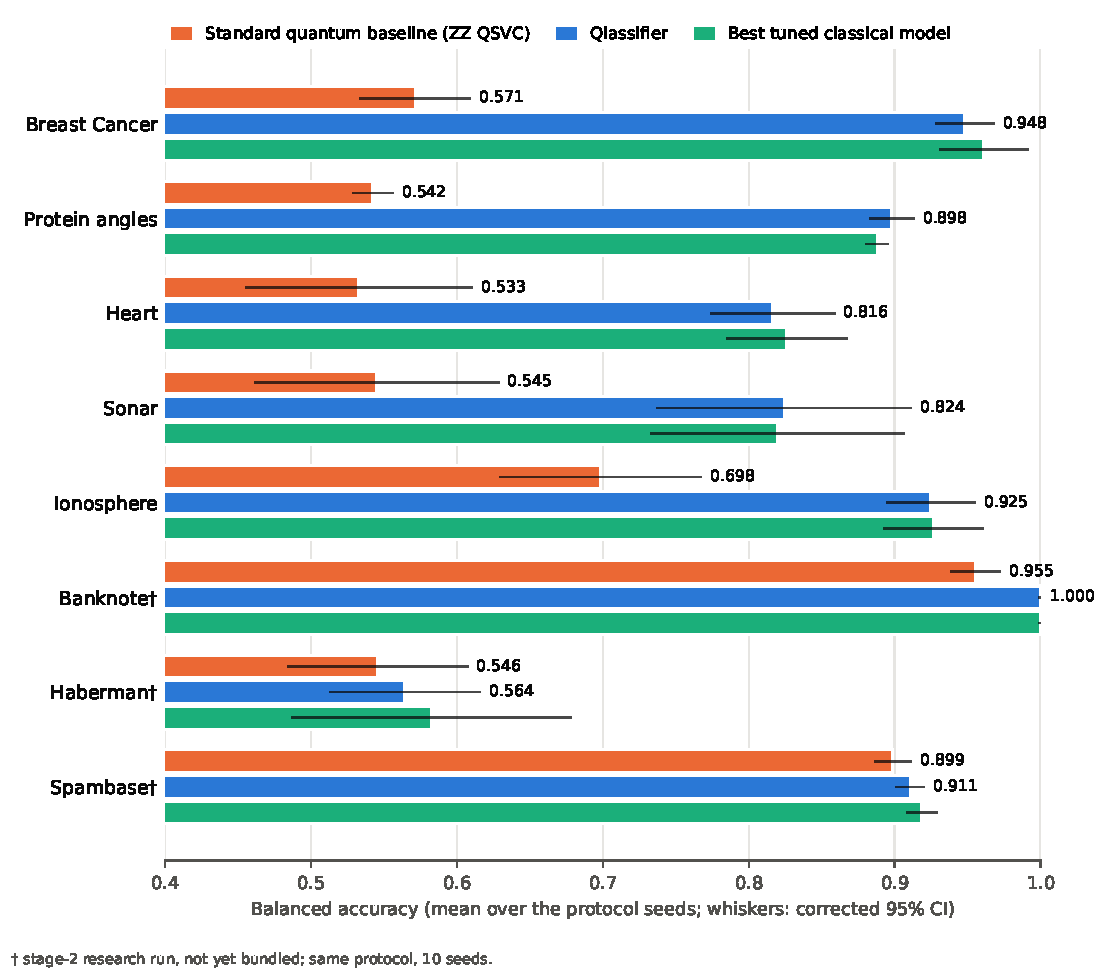
\includegraphics[width=0.92\textwidth]{wins}
\caption{Balanced accuracy of Qlassifier against the standard quantum baseline (ZZ feature
map QSVC) and the best tuned classical model on every dataset of this paper. Means over the protocol's seeds, whiskers
are corrected confidence intervals. Datasets are sorted by Qlassifier's gain over the standard baseline. Spambase,
Banknote and Haberman are the additional datasets of Sec.~\ref{sec:stage2data}. Script:
\code{scripts/wins\_chart.py}.}
\label{fig:wins}
\end{figure*}

Quantum kernel methods are the most common entry point to quantum machine learning on real data. The standard recipe
is a support vector classifier on the fidelity kernel of the ZZ feature map~\cite{havlicek2018supervised}, as shipped
by Qiskit~\cite{javadiabhari2024quantum}. On real data this recipe often collapses. In our harness it reaches a mean
BA of \val{bc.zz.ba} on Breast Cancer, \val{iono.zz.ba} on Ionosphere, \val{sonar.zz.ba} on Sonar and \val{heart.zz.ba}
on Heart, where 0.5 is chance (Fig.~\ref{fig:wins}).

The known fixes are expensive. Tuning the input scale (the ``bandwidth'') makes fidelity kernels
work~\cite{shaydulin2021importance,canatar2022bandwidth,egginger2023a}, but on a device each candidate bandwidth needs a
new Gram matrix, with one circuit per pair of samples. Training the kernel itself~\cite{hubregtsen2021training,glick2021covariant} needs a new
Gram matrix at every optimisation step. Deep entangled feature maps also lose most of their signal on today's
hardware: the pinned ZZ circuit needs \val{bc.twoq.zz.min} to \val{bc.twoq.zz.max} two-qubit gates on
\val{bc.qubits.zz} qubits after transpilation to IBM devices (Table~\ref{tab:cost}). Finally, well-tuned quantum kernels
tend to behave like classical RBF kernels~\cite{florezablan2025on,bowles2024better}, and public tabular data rarely
leaves room for a quantum edge~\cite{mancilla2026the}.

Qlassifier keeps its circuits fixed and tunes only after the measurement. This paper reports:
\begin{itemize}
\item a product-state kernel classifier with zero-circuit self-tuning and a three-setting hardware protocol
  (Sec.~\ref{sec:method});
\item a geometry mode for angle-valued data, with its exact classical twin (Sec.~\ref{sec:geometry});
\item a benchmark against the standard classical and quantum baselines and four published quantum kernels, included in
  the library (Sec.~\ref{sec:protocol});
\item results on accuracy, noise robustness, cost and run time, with confidence intervals (Sec.~\ref{sec:results}),
  and the limitations (Sec.~\ref{sec:limits});
\item a run on an IBM Heron processor, compared with a prediction written before submission
  (Sec.~\ref{sec:hardware}), a noise sweep to \val{sweep.max} times the device error rates (Sec.~\ref{sec:sweep}) and
  three further datasets (Sec.~\ref{sec:stage2data}).
\end{itemize}
The library is open source (MIT licence) at \repo. All numbers in this paper are generated from the saved benchmark
results by a script; Sec.~\ref{sec:repro} shows how to rerun them.

% ---------------------------------------------------------------------------------------------------------------------
\section{Method}
\label{sec:method}

\subsection{Core encoding}
Each plain feature is standardised with the mean and standard deviation of the training rows, giving $\tilde{x}$.
Qubit $q$ carries the pair $(\tilde x_{2q}, \tilde x_{2q+1})$:
\begin{equation}
\ket{\psi_q(\mathbf{x})} = R_Y(c_0 \tilde x_{2q+1})\, R_X(c_0 \tilde x_{2q})\, \ket{0},
\label{eq:encoding}
\end{equation}
so $d$ features need $n = \lceil d/2 \rceil$ qubits and no two-qubit gate. The angle scale $c_0 = 2/\sqrt{\max(d, 8)}$
is fixed, not tuned. It keeps standardised values inside one period of the rotation (the cap at 8 avoids folding at
small $d$). With $a = c_0 \tilde x_{2q}$ and $b = c_0 \tilde x_{2q+1}$, the Bloch vector of qubit $q$ is
\begin{equation}
\mathbf{r}_q = (\cos a \sin b,\; -\sin a,\; \cos a \cos b).
\end{equation}
This dense angle encoding is known~\cite{larose2020robust,stoudenmire2016supervised}; what follows is how we read it
out and tune it.

\subsection{Readout and kernel}
Three circuits per sample measure all qubits in the $X$, $Y$ and $Z$ bases, which gives $F(\mathbf{x}) =
(\mathbf{r}_1, \dots, \mathbf{r}_n) \in \mathbb{R}^{3n}$. The kernel is Gaussian on these features:
\begin{equation}
k(\mathbf{x}, \mathbf{x}') = e^{-\gamma \lVert F(\mathbf{x}) - F(\mathbf{x}') \rVert^2}
= \prod_{q=1}^{n} e^{-4\gamma\, [1 - f_q(\mathbf{x}, \mathbf{x}')]},
\label{eq:kernel}
\end{equation}
where $f_q = (1 + \mathbf{r}_q \cdot \mathbf{r}'_q)/2$ is the single-qubit fidelity, $\gamma = g\, \gamma_0$ and
$\gamma_0 = 1/\sum_k \mathrm{Var}(F_k)$ over the training rows. This is a projected quantum
kernel~\cite{huang2020power} on a product state, or equivalently a tempered fidelity kernel. A support vector machine
uses the precomputed Gram matrix. For small angles $\lVert F(\mathbf{x}) - F(\mathbf{x}') \rVert^2 \approx c_0^2
\lVert \tilde{\mathbf{x}} - \tilde{\mathbf{x}}' \rVert^2$, so the core kernel is close to an RBF kernel. This explains
the ties with RBF-SVM below.

\subsection{Self-tuning at zero circuits}
The two hyperparameters act after the measurement: $g$ scales the kernel width and $C$ the margin. Qlassifier therefore
tunes them on exact (closed-form) features and never runs a circuit to tune. It uses \val{protocol.folds}-fold stratified
cross-validation on the training rows, scored by balanced accuracy, over a ridge-following
grid~\cite{keerthi2003asymptotic}: $g \in \{4^{-3}, \dots, 4^{2}\}$ and $C = \tilde C / g$ with $\tilde C \in
\{10^{-1}, \dots, 10^{3}\}$, \val{protocol.configs} configurations in total. Ties go to the first configuration in grid
order. A device measures only the final features of the training and test rows. Probabilities come from a Platt
sigmoid fitted on out-of-fold decision values.

\subsection{Geometry mode for angle-valued data}
\label{sec:geometry}
Some columns are angles: dihedral angles, wind directions, times of day, longitudes. A periodic column $x$ with period
$P$ gets its own qubit, $\ket{\psi(x)} = R_Y(t)\ket{0}$ with $t = 2\pi x/P$, so $\mathbf{r} = (\sin t, 0, \cos t)$.
The kernel factor of that qubit is
\begin{equation}
e^{-\gamma \lVert \mathbf{r} - \mathbf{r}' \rVert^2} = e^{-2\gamma\, [1 - \cos(t - t')]},
\end{equation}
a von~Mises kernel with concentration $2\gamma$~\cite{sra2016directional,pewsey2020recent}. It has no seam: $359^\circ$
and $1^\circ$ are neighbours. A (latitude, longitude) pair maps to one qubit with $R_Z(\varphi) R_Y(\theta)$,
$\theta = 90^\circ - \text{latitude}$, $\varphi = \text{longitude}$; its Bloch vector is the direction itself and its
kernel factor is a von~Mises--Fisher kernel on the sphere.

Two circles cannot share a qubit. The map of Eq.~(\ref{eq:encoding}) sends $(a, b)$ and $(\pi - a, b + \pi)$ to the same
Bloch vector, because the torus does not embed in the sphere. Geometry mode therefore uses one qubit per circle, more
than the $\lceil d/2 \rceil$ of the core encoding, and our hardware target counts it by this rule
(Sec.~\ref{sec:limits}). It is still free of two-qubit gates.

\textit{Classical twin.} When every column is angular, the geometry-mode Gram matrix equals that of an RBF kernel on
hand-made features: $(\sin t, \cos t)$ per circle and the unit vector per direction. Both give the same squared
distances, and the zero-variance $Y$ components leave $\gamma_0$ unchanged. The library tests this identity to
$10^{-12}$. Any gain of geometry mode therefore comes from the geometric prior, which a classical model can also use through
feature engineering. We report the twin next to every geometry-mode result.

\subsection{Execution on devices}
The \code{backend} parameter selects where Bloch vectors come from: the closed form (\code{"exact"}, the default),
binomial shot sampling of each Pauli expectation (\code{"shots"}, the exact law for product states) or the noise models
of IBM devices (\code{"fake\_torino"}, \code{"fake\_fez"}, \code{"fake\_brisbane"}: Heron r1, Heron r2 and Eagle r3,
simulated with Qiskit Aer). Circuits are transpiled once at optimisation level 3; the $X$ and $Y$ circuits reuse the
physical qubits chosen for the $Z$ circuit. Each component is estimated as $1 - 2P(1)$ from \val{noise.shots} shots, and
each measured Bloch vector is renormalised to unit length, a per-qubit mitigation that costs no extra circuit. The
circuits are product states, and the device noise models act qubit by qubit: single-qubit gate errors and readout
errors, no crosstalk, no idle noise. So the library simulates each qubit alone, on the physical qubit that the
full-register transpilation chose, at a cost linear in the number of qubits. This reproduces the full-register
marginals exactly: over \val{e14.marginals} marginals the largest difference was \val{e14.maxdiff} (experiment e14 in
the repository). The library checks these conditions at run time and otherwise simulates
the full register.

\subsection{Resources}
Per circuit, the core encoding needs $\lceil d/2 \rceil$ qubits (\val{bc.qubits} for $d = 8$), no two-qubit gate and a
transpiled depth of \val{bc.depth} on the three devices. Training and prediction need 3 circuits per sample:
\val{bc.circuits} circuits for the \val{bc.rows} Breast Cancer rows. Tuning needs none. Classically, the Gram matrix
costs $O(N^2 n)$ time and $N^2$ memory.

% ---------------------------------------------------------------------------------------------------------------------
\section{Benchmark protocol}
\label{sec:protocol}

The benchmark follows the fair-comparison rules of the Qiskit Fall Fest 2026 QML challenge and was fixed before the
method search (\code{experiments/classifier/README.md}, Sec.~2, in the repository). It ships inside the library: \code{qlassifier benchmark}
reruns it.

\textit{Data.} Table~\ref{tab:datasets} lists the five bundled datasets: four UCI
datasets~\cite{street1993nuclear,sigillito1989classification,gorman1988analysis,detrano1989international} and protein
backbone dihedral angles from the Protein Data Bank~\cite{berman2000protein}. The protein task asks whether residue $i$
lies in a $\beta$-strand, from the $(\phi, \psi)$ angles of residues $i-2$ to $i+2$. The positive class is always the
minority class.

\begin{table*}[t]
\centering
\caption{Bundled datasets. UCI sets: every model gets the same \val{protocol.features} PCA features, fitted inside every
training fold. Protein: every model gets the same \val{protein.features} raw angles; geometry mode declares them as
circles of period $360^\circ$. Chain-grouped splits keep every protein chain on one side of each split.}
\label{tab:datasets}
{\small% Generated by scripts/paper_tables.py from the saved results. Do not edit: rerun the script.
\begin{tabular}{lrrlllp{0.22\textwidth}}
\toprule
Dataset & Rows & Features & Positive class & Features used & Split & Licence \\
\midrule
Breast Cancer & 569 & 30 & malignant (212) & PCA to 8 & stratified & CC BY 4.0 (UCI); BSD-3-Clause (scikit-learn copy) \\
Ionosphere & 351 & 33 & bad (126) & PCA to 8 & stratified & CC BY 4.0 \\
Sonar & 208 & 60 & rock (97) & PCA to 8 & stratified & CC BY 4.0 \\
Heart & 297 & 13 & disease (137) & PCA to 8 & stratified & CC BY 4.0 \\
Protein angles & 4,000 & 10 & strand (996) & 10 angles (raw) & chain-grouped & CC0 1.0 \\
\bottomrule
\end{tabular}
}
\end{table*}

\textit{Splits.} Seeds 0 to \val{protocol.seed.last}: one stratified \val{protocol.testshare}\% test split per seed
(protein: grouped by PDB chain), identical for every model. All preprocessing is fitted on training rows only.

\textit{Models.} Majority class; logistic regression, RBF-SVM, random forest, histogram gradient boosting and an MLP
(scikit-learn~\cite{pedregosa2012scikitlearn}); the pinned standard quantum baseline, a QSVC on the fidelity kernel of
the ZZ feature map (2 repetitions, full entanglement, inputs scaled to $[0, \pi]$); four published quantum kernels
re-implemented under the same protocol: the bandwidth-tuned fidelity kernel with full and linear
entanglement~\cite{shaydulin2021importance,canatar2022bandwidth}, the projected quantum kernel~\cite{huang2020power}
and the separable kernel~\cite{bowles2024better}; Qlassifier; and on the protein data the classical twin as a control.
Exact simulation is used for every quantum model in the leaderboard.

\textit{Tuning.} Every tuned model gets \val{protocol.configs} configurations, scored by \val{protocol.folds}-fold
cross-validation on balanced accuracy inside the training split, then refits on the whole training split. The pinned ZZ
baseline keeps its \val{protocol.configs.zz} values of $C$. No test label is seen before the final evaluation.

\textit{Statistics.} Repeated random splits overlap, so a plain $t$-test over seeds is anti-conservative. Every interval
is a corrected resampled $t$ interval~\cite{nadeau2003inference},
\begin{equation}
\mathrm{SE} = s \sqrt{1/J + n_\text{test}/n_\text{train}},
\end{equation}
with $J$ seeds and $J-1$ degrees of freedom. Paired differences (Qlassifier minus a model) use the same correction. A
model is ``tied with the best'' when the \val{protocol.cilevel}\% interval of its paired difference to the top model
contains 0. The best classical model is chosen after the fact, which is conservative for a quantum claim. The paired
intervals (one per model and dataset) are reported without a multiple-comparison correction: they describe ties, not
discoveries, and each target rests on one pre-registered test (the earlier protein tests used Bonferroni-corrected
intervals, Table~\ref{tab:history}). Reading a tie from an uncorrected interval is conservative for a quantum win.

\textit{Grid edges.} Equal effort is counted in configurations, not seconds. The chosen configuration sits on an edge of
the grid for at least half the seeds for \val{edge.list} (share of seeds, datasets); Qlassifier's largest share is
\val{edge.qlassifier.max} (\val{edge.qlassifier.where}). The budget is equal, but a wider grid could move these
models, in either direction; the per-seed edge flag is in every \code{runs.csv}.

\textit{Noise study.} Part A runs Qlassifier on every dataset (all rows, seeds \val{noise.a.first} to
\val{noise.a.last}) on the shot sampler and the three device models. Part B compares Qlassifier with the bandwidth-tuned fidelity kernel (linear), the projected kernel and
the separable kernel on identical Breast Cancer subsets (\val{noise.b.ntrain} training and \val{noise.b.ntest} test
rows, \val{noise.b.seeds} seeds), because fidelity kernels need one circuit per pair of rows. Hyperparameters come
from exact-mode tuning; nothing is re-tuned on noisy data.

\textit{Cost study.} Each quantum model's circuit is transpiled to the three devices (median of 3 transpiler seeds).
Circuit counts cover training and prediction at the chosen configuration, plus, for models whose hyperparameters change
the circuit, the on-device bandwidth search.

\textit{Targets.} Ten targets, BT-1 to BT-10, were fixed before the benchmark ran. The library
evaluates them from the saved results (Table~\ref{tab:targets}).

% ---------------------------------------------------------------------------------------------------------------------
\section{Results}
\label{sec:results}

\begin{table*}[t]
\centering
\caption{Balanced accuracy, mean $\pm$ standard deviation over \val{bc.seeds} seeds. Bold: top mean per dataset.
$^{\approx}$: statistically tied with the top model (corrected \val{protocol.cilevel}\% CI of the paired difference
contains 0). The classical twin exists only for the geometry-mode dataset.}
\label{tab:leaderboard}
{\small% Generated by scripts/paper_tables.py from the saved results. Do not edit: rerun the script.
\begin{tabular}{lccccc}
\toprule
Model & Breast Cancer & Ionosphere & Sonar & Heart & Protein angles \\
\midrule
\textbf{Qlassifier} & 0.948 $\pm$ 0.012$^{\approx}$ & 0.925 $\pm$ 0.018$^{\approx}$ & \textbf{0.824 $\pm$ 0.053}$^{\approx}$ & 0.816 $\pm$ 0.026$^{\approx}$ & \textbf{0.898 $\pm$ 0.009}$^{\approx}$ \\
Classical twin & --- & --- & --- & --- & \textbf{0.898 $\pm$ 0.009}$^{\approx}$ \\
\midrule
ZZ QSVC & 0.571 $\pm$ 0.023 & 0.698 $\pm$ 0.042 & 0.545 $\pm$ 0.051 & 0.533 $\pm$ 0.047 & 0.542 $\pm$ 0.008 \\
FQK-bw full & 0.944 $\pm$ 0.018$^{\approx}$ & 0.891 $\pm$ 0.031$^{\approx}$ & 0.800 $\pm$ 0.036$^{\approx}$ & 0.823 $\pm$ 0.029$^{\approx}$ & 0.878 $\pm$ 0.013 \\
FQK-bw linear & 0.946 $\pm$ 0.020$^{\approx}$ & 0.904 $\pm$ 0.031$^{\approx}$ & 0.772 $\pm$ 0.037$^{\approx}$ & 0.800 $\pm$ 0.053$^{\approx}$ & 0.877 $\pm$ 0.011 \\
PQK & 0.950 $\pm$ 0.014$^{\approx}$ & 0.900 $\pm$ 0.035$^{\approx}$ & 0.806 $\pm$ 0.043$^{\approx}$ & 0.793 $\pm$ 0.043$^{\approx}$ & 0.878 $\pm$ 0.009 \\
Separable & 0.952 $\pm$ 0.015$^{\approx}$ & 0.898 $\pm$ 0.031$^{\approx}$ & 0.805 $\pm$ 0.040$^{\approx}$ & \textbf{0.826 $\pm$ 0.025}$^{\approx}$ & 0.888 $\pm$ 0.008$^{\approx}$ \\
\midrule
Logistic regression & 0.954 $\pm$ 0.018$^{\approx}$ & 0.845 $\pm$ 0.029 & 0.721 $\pm$ 0.046 & \textbf{0.826 $\pm$ 0.025}$^{\approx}$ & 0.838 $\pm$ 0.010 \\
RBF-SVM & 0.949 $\pm$ 0.012$^{\approx}$ & \textbf{0.926 $\pm$ 0.021}$^{\approx}$ & 0.814 $\pm$ 0.055$^{\approx}$ & 0.820 $\pm$ 0.025$^{\approx}$ & 0.877 $\pm$ 0.011 \\
Random forest & 0.923 $\pm$ 0.021 & 0.905 $\pm$ 0.026$^{\approx}$ & 0.784 $\pm$ 0.072$^{\approx}$ & 0.792 $\pm$ 0.030$^{\approx}$ & 0.883 $\pm$ 0.007 \\
Gradient boosting & 0.948 $\pm$ 0.018$^{\approx}$ & 0.886 $\pm$ 0.024$^{\approx}$ & 0.754 $\pm$ 0.040$^{\approx}$ & 0.784 $\pm$ 0.031$^{\approx}$ & 0.888 $\pm$ 0.005$^{\approx}$ \\
MLP & \textbf{0.961 $\pm$ 0.019}$^{\approx}$ & 0.915 $\pm$ 0.030$^{\approx}$ & 0.820 $\pm$ 0.052$^{\approx}$ & 0.820 $\pm$ 0.027$^{\approx}$ & 0.884 $\pm$ 0.008$^{\approx}$ \\
\midrule
Majority class & 0.500 $\pm$ 0.000 & 0.500 $\pm$ 0.000 & 0.500 $\pm$ 0.000 & 0.500 $\pm$ 0.000 & 0.500 $\pm$ 0.000 \\
\bottomrule
\end{tabular}
}
\end{table*}

\begin{table*}[t]
\centering
\caption{Qlassifier against the standard quantum baseline and the best tuned classical model. $\Delta$ = Qlassifier
minus the other model, in percentage points (pp), with corrected \val{protocol.cilevel}\% CIs; wins = seeds on which
Qlassifier is higher.}
\label{tab:comparisons}
{\footnotesize% Generated by scripts/paper_tables.py from the saved results. Do not edit: rerun the script.
\begin{tabular}{lccclc}
\toprule
 & Qlassifier BA & \multicolumn{2}{c}{$\Delta$ vs ZZ QSVC} & \multicolumn{2}{c}{$\Delta$ vs best classical} \\
Dataset & mean [95\% CI] & pp [95\% CI] & wins & model & pp [95\% CI] (wins) \\
\midrule
Breast Cancer & 0.948 [0.928, 0.968] & +37.6 [+34.6, +40.7] & 10/10 & MLP & $-$1.3 [$-$3.1, +0.5] (0/10) \\
Ionosphere & 0.925 [0.894, 0.955] & +22.6 [+13.9, +31.4] & 10/10 & RBF-SVM & $-$0.2 [$-$3.1, +2.7] (5/10) \\
Sonar & 0.824 [0.737, 0.912] & +27.9 [+14.7, +41.2] & 10/10 & MLP & +0.5 [$-$8.5, +9.5] (6/10) \\
Heart & 0.816 [0.773, 0.859] & +28.3 [+20.4, +36.3] & 10/10 & Logistic regression & $-$1.0 [$-$3.1, +1.2] (2/10) \\
Protein angles & 0.898 [0.883, 0.913] & +35.5 [+34.6, +36.5] & 10/10 & Gradient boosting & +1.0 [$-$0.2, +2.2] (10/10) \\
\bottomrule
\end{tabular}
}
\end{table*}

\subsection{Against the standard quantum baseline}
Qlassifier beats the pinned ZZ QSVC on every dataset and every seed (Table~\ref{tab:comparisons}): by
\val{uci.vszz.min} to \val{uci.vszz.max}\pp\ BA on the four UCI datasets and by \val{protein.vszz}\pp\ on the protein
angles. On Breast Cancer the accuracy rises from \val{bc.zz.acc} to \val{bc.acc} (BT-1). The ZZ baseline is not
broken by a bug. Its input scale is fixed, so on \val{bc.qubits.zz} qubits its kernel matrix is close to the identity
on real data, and tuning $C$ cannot repair that~\cite{shaydulin2021importance,canatar2022bandwidth}.

\subsection{Against other quantum models}
Averaged over the four UCI datasets, Qlassifier has the highest mean BA of the six quantum models in the harness
(\val{uci.mean.qlassifier}; next: \val{uci.mean.runnerup}, \val{uci.mean.runnerup.ba}; BT-5). The differences between
the good quantum kernels are small and mostly inside the CIs.

\begin{figure*}[t]
\centering
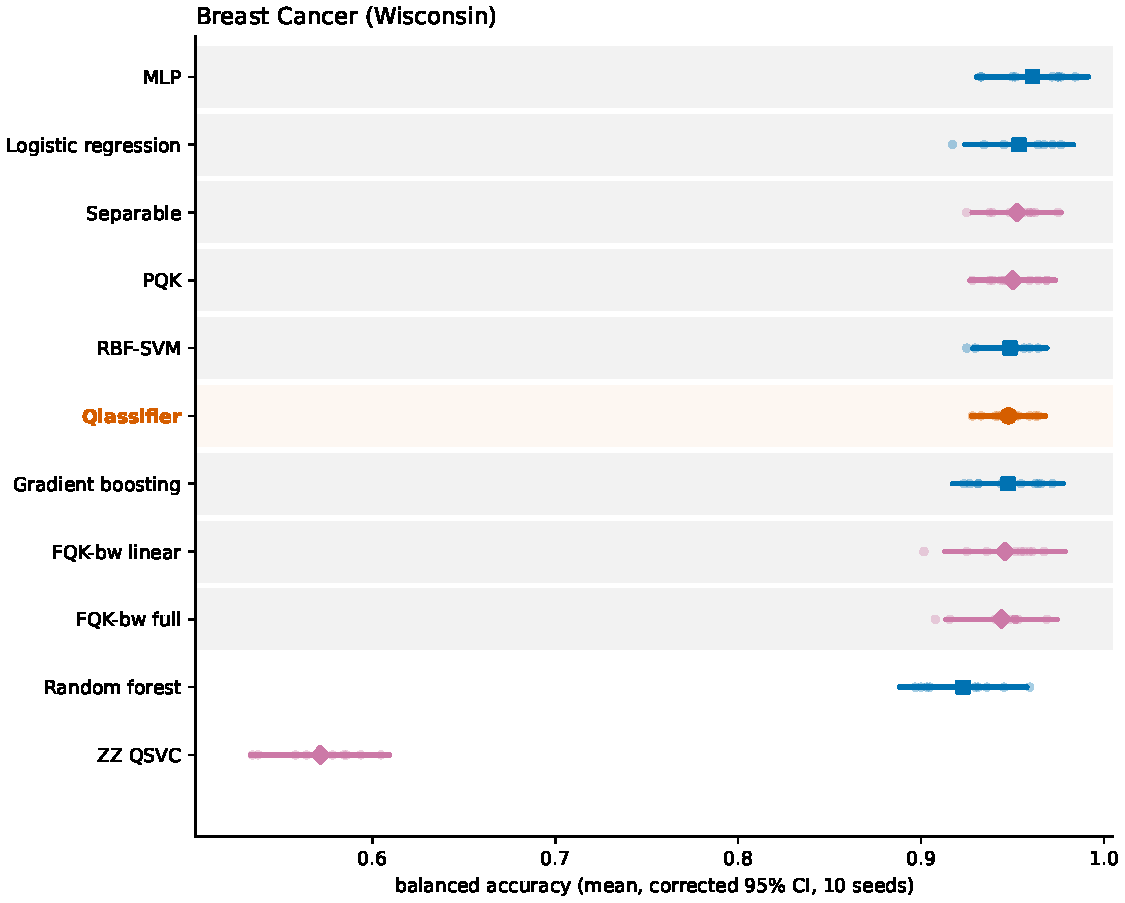
\includegraphics[width=0.62\textwidth]{breast_cancer-leaderboard}
\caption{Breast Cancer leaderboard: per-seed BA (dots), corrected \val{protocol.cilevel}\% CI (bar) and mean (marker) for every model.
Qlassifier (vermillion) sits inside the band tied with the best, far above the ZZ QSVC.}
\label{fig:bc}
\end{figure*}

\subsection{Against tuned classical models}
On every dataset Qlassifier is statistically tied with the best tuned classical model (Table~\ref{tab:comparisons}).
The mean differences range from \val{all.vsbest.min} to \val{all.vsbest.max}\pp. With \val{bc.seeds} seeds and test
sets of \val{all.ntest.min} to \val{all.ntest.max} rows, the corrected \val{protocol.cilevel}\% half-widths of these differences are
\val{all.halfwidth.min} to \val{all.halfwidth.max}\pp, so differences of about one point cannot be resolved. Ties are
the expected outcome on generic tabular data, as the small-angle limit of Eq.~(\ref{eq:kernel}) predicts.

\subsection{Geometry mode on protein angles}
\label{sec:protein}
On the protein angles, geometry mode ranks \val{protein.rank} by mean BA (\val{protein.ba} $\pm$ \val{protein.ba.sd}).
Its difference to the best tuned classical model, \val{protein.best}, is \val{protein.vsbest}\pp\ (\val{protocol.cilevel}\% CI
\val{protein.vsbest.ci}, \val{protein.vsbest.wins} seeds): \val{protein.vsbest.word}. Against RBF-SVM the difference is
\val{protein.vs.rbfsvm}\pp\ (CI \val{protein.vs.rbfsvm.ci}), against logistic regression
\val{protein.vs.logisticregression}\pp\ (CI \val{protein.vs.logisticregression.ci}). Its classical twin scores
\val{protein.twin.ba}: \val{protein.twin.identical}. The protein data was chosen in an earlier search, so these seeds
are a confirmation run; Table~\ref{tab:history} lists every look at this question, including the leaky residue-level
split that first suggested a significant win.

\begin{figure*}[t]
\centering
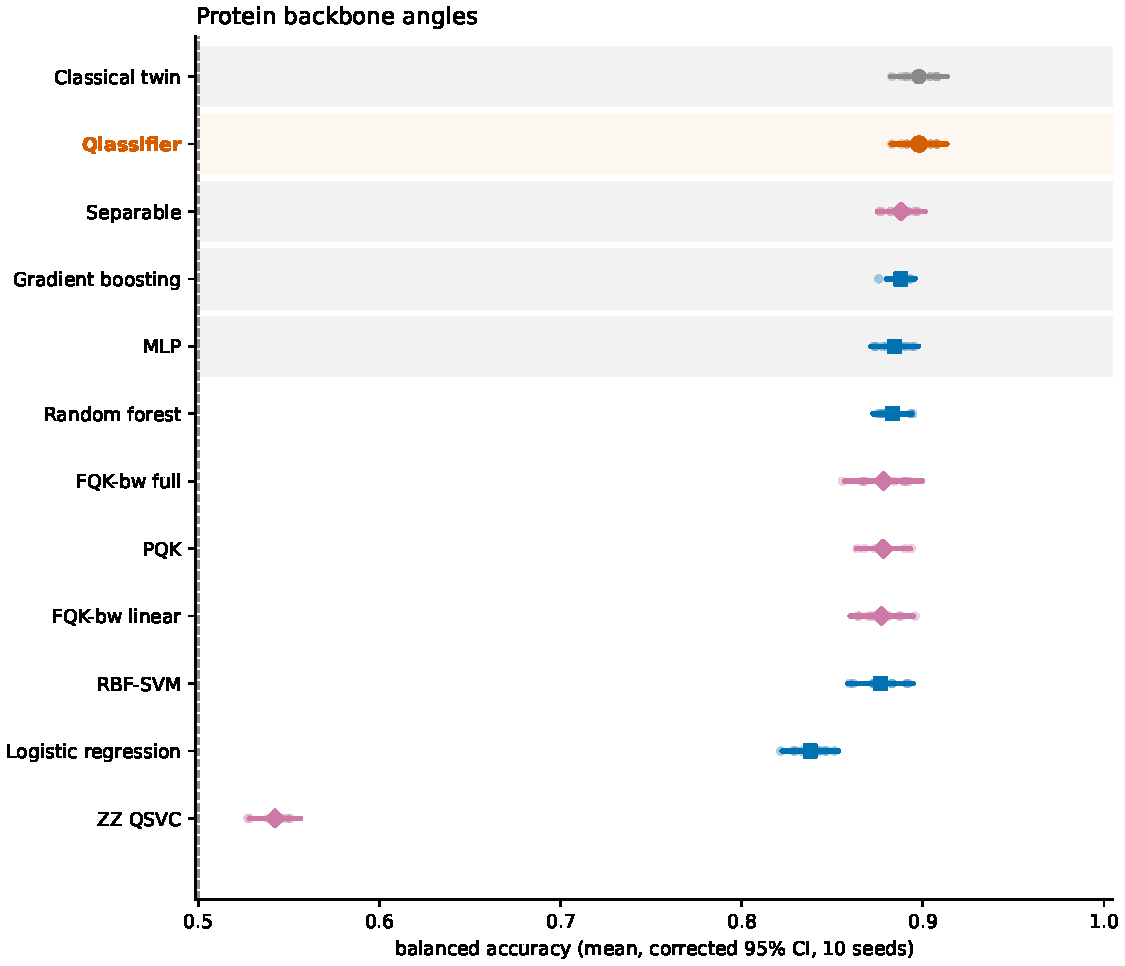
\includegraphics[width=0.62\textwidth]{protein_angles-leaderboard}
\caption{Protein backbone angles (chain-grouped splits): leaderboard as in Fig.~\ref{fig:bc}. The classical twin
(grey) computes the same Gram matrix as geometry mode from hand-made $(\sin, \cos)$ features.}
\label{fig:protein}
\end{figure*}

\begin{table*}[t]
\centering
\caption{The tuned-classical target (BT-6) on protein data, every run. Geometry mode minus the best classical model,
in pp. e07: residue-level splits, which share protein chains between training and test. e11, e12: chain-grouped,
pre-registered; e12 used Bonferroni-corrected \val{e12.div6.level}\% CIs for its two hypotheses. This paper: the run reported here.}
\label{tab:history}
{\small% Generated by scripts/paper_tables.py from the saved results. Do not edit: rerun the script.
\begin{tabular}{llllccc}
\toprule
Run & Data, split & Seeds & Best classical & Qlassifier & $\Delta$ BA, pp [CI] & CI level \\
\midrule
e07 & protein\_strands, residue-level split & 200--209 & MLP 0.870 & 0.884 & +1.4 [+0.3, +2.4] & 95\% \\
e11 & protein\_strands, chain-grouped & 200--209 & MLP 0.872 & 0.879 & +0.7 [$-$0.6, +2.1] & 95\% \\
e12 & protein\_div6, chain-grouped & 300--309 & MLP 0.887 & 0.889 & +0.25 [$-$1.13, +1.62] & 97.5\% \\
e12 & protein\_div10, chain-grouped & 300--309 & Gradient boosting 0.889 & 0.897 & +0.81 [$-$0.61, +2.23] & 97.5\% \\
this paper & protein\_angles, chain-grouped & 0--9 & Gradient boosting 0.888 & 0.898 & +1.0 [$-$0.2, +2.2] & 95\% \\
\bottomrule
\end{tabular}
}
\end{table*}

\subsection{Noise}
Table~\ref{tab:noise} gives the accuracy lost from exact simulation to each noise model (positive: lost; negative:
gained). Over the five datasets and three device models, Qlassifier's mean change lies between \val{noise.min} and
\val{noise.max}\pp, and its kernel keeps a Pearson correlation of at least \val{noise.r.min} with the exact kernel.
On the paired Part~B subsets, at \val{noise.shots} shots, the bandwidth-tuned fidelity kernel loses \val{bc.noiseb.fqk.min} to
\val{bc.noiseb.fqk.max}\pp, the separable kernel up to \val{bc.noiseb.separable.max}\pp, and Qlassifier at most
\val{bc.noiseb.qlassifier.max}\pp\ (BT-9). Most of the fidelity kernel's loss is sampling noise, not gate error: with
device noise switched off it already loses \val{sweep.fqk.drop0}\pp\ (Sec.~\ref{sec:sweep}). These are means over seeds; the worst single seed lost
\val{noise.worst}\pp\ in Part~A (\val{noise.worst.dataset}) and \val{bc.noiseb.qlassifier.worst}\pp\ in Part~B.
Fig.~\ref{fig:noise} shows Breast Cancer.

On Breast Cancer the three device models give the same mean loss,
\val{bc.noise.torino} / \val{bc.noise.fez} / \val{bc.noise.brisbane}\pp: with \val{noise.shots} shots and a shared
sampler seed, their estimates coincide to the flip, so device differences on this data lie below the shot resolution.
An earlier run of the same study, which simulated the whole register, measured \val{e05.torino} /
\val{e05.fez} / \val{e05.brisbane}\pp\ (e05 in the repository). The shipped run samples each qubit alone and draws a
different random stream from the simulator, so the two differ by one shot-noise resampling; both stay below
\val{e05.max}\pp.

\begin{table*}[t]
\centering
\caption{Accuracy lost under noise, in pp: mean over seeds (worst seed in brackets); \val{noise.shots} shots.
Part A: Qlassifier on all rows, \val{noise.a.seeds} seeds. Part B: four quantum models on identical Breast Cancer
subsets. Kernel $r$: lowest mean Pearson correlation of the noisy and exact kernels over the noise models.}
\label{tab:noise}
{\small% Generated by scripts/paper_tables.py from the saved results. Do not edit: rerun the script.
\begin{tabular}{llccccc}
\toprule
Part & Model, dataset & shots & Torino & Fez & Brisbane & kernel $r$ (min) \\
\midrule
A & Qlassifier, Breast Cancer & $-$0.12 (+0.6) & +0.12 (+0.6) & +0.12 (+0.6) & +0.12 (+0.6) & 0.9983 \\
A & Qlassifier, Ionosphere & $-$0.19 (0.0) & $-$0.38 (+0.9) & $-$0.75 (+0.9) & $-$0.38 (+0.9) & 0.9973 \\
A & Qlassifier, Sonar & $-$0.32 (+1.6) & $-$0.32 (0.0) & $-$0.63 (0.0) & $-$0.63 (0.0) & 0.9968 \\
A & Qlassifier, Heart & $-$1.56 (0.0) & $-$0.89 (0.0) & $-$1.33 (0.0) & $-$1.33 (0.0) & 0.9980 \\
A & Qlassifier, Protein angles & +0.18 (+0.4) & +0.17 (+0.4) & +0.17 (+0.4) & +0.19 (+0.3) & 0.9998 \\
\midrule
B & Qlassifier, Breast Cancer 60/40 & --- & +0.8 (+2.5) & +0.8 (+2.5) & +0.8 (+2.5) & 0.9981 \\
B & FQK-bw linear, Breast Cancer 60/40 & --- & +22.5 (+27.5) & +20.0 (+27.5) & +17.5 (+35.0) & 0.9069 \\
B & PQK, Breast Cancer 60/40 & --- & 0.0 (+2.5) & +1.7 (+7.5) & 0.0 (0.0) & 0.9821 \\
B & Separable, Breast Cancer 60/40 & --- & +14.2 (+30.0) & +13.3 (+30.0) & +10.8 (+22.5) & 0.8673 \\
\bottomrule
\end{tabular}
}
\end{table*}

\begin{figure*}[t]
\centering
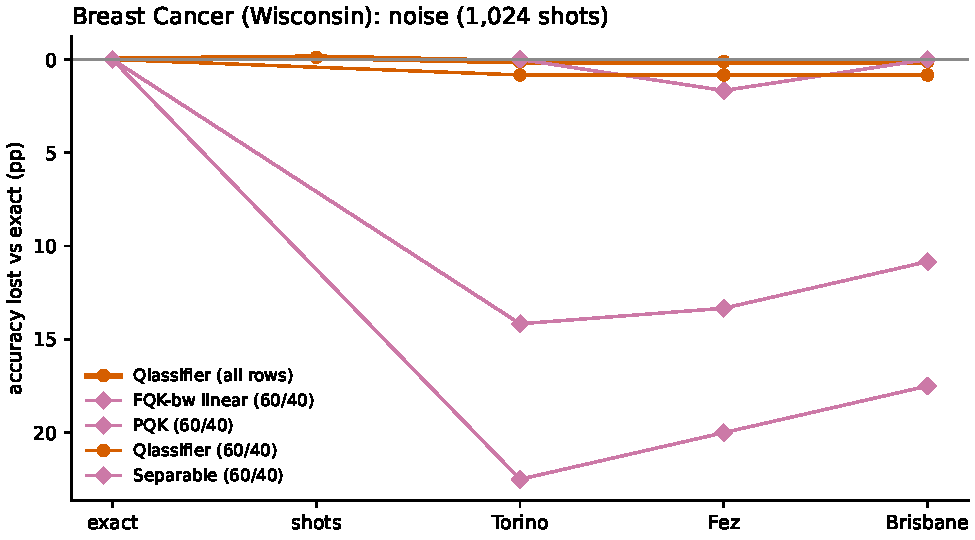
\includegraphics[width=0.7\textwidth]{breast_cancer-noise}
\caption{Accuracy lost from exact simulation to shot noise and three IBM device noise models, Breast Cancer. Thick
line: Qlassifier on all rows (Part A). Thin lines: the Part~B subsets.}
\label{fig:noise}
\end{figure*}

\subsection{Noise scaled beyond the device}
\label{sec:sweep}
We scaled every error channel of the FakeFez model (gate and
readout errors multiplied by $s$, $T_1$ and $T_2$ divided by $s$) for $s \in \{\val{sweep.scales}\}$ and reran Breast
Cancer at \val{noise.shots} shots. Qlassifier's mean accuracy loss is \val{sweep.q.drop1}\pp\ at $s = 1$ and
\val{sweep.q.drop3}\pp\ at $s = \val{sweep.max}$ (worst seed \val{sweep.q.drop1.worst}\pp; \val{sweep.a.seeds} seeds,
all rows), and its kernel keeps $r = \val{sweep.q.r3}$ with the exact kernel at $s = \val{sweep.max}$. On the paired
subsets (\val{sweep.b.seeds} seeds) the mean accuracy over the sweep is \val{sweep.auc.q} for Qlassifier,
\val{sweep.auc.fqk} for the bandwidth-tuned fidelity kernel and \val{sweep.auc.zz} for the ZZ baseline
(\val{sweep.zz.seeds} seeds at $s \in \{0, 1, 3\}$), Fig.~\ref{fig:sweep}. The fidelity kernel loses
\val{sweep.fqk.drop0}\pp\ already at $s = 0$, from \val{noise.shots}-shot sampling alone, and \val{sweep.fqk.drop3}\pp\ at
$s = \val{sweep.max}$: its noise loss is mostly shot noise, the price of estimating one fidelity per pair of samples. The
ZZ classifier stays at the majority class throughout while its kernel correlation with the exact kernel falls from
\val{sweep.zz.r0} to \val{sweep.zz.r3}. Qlassifier's curve is flat because, for depth-\val{hw.depth} single-qubit circuits,
device noise lies far below the shot resolution. A scaled noise model does not replace a hardware run
(Sec.~\ref{sec:hardware}).

\begin{figure}[t]
\centering
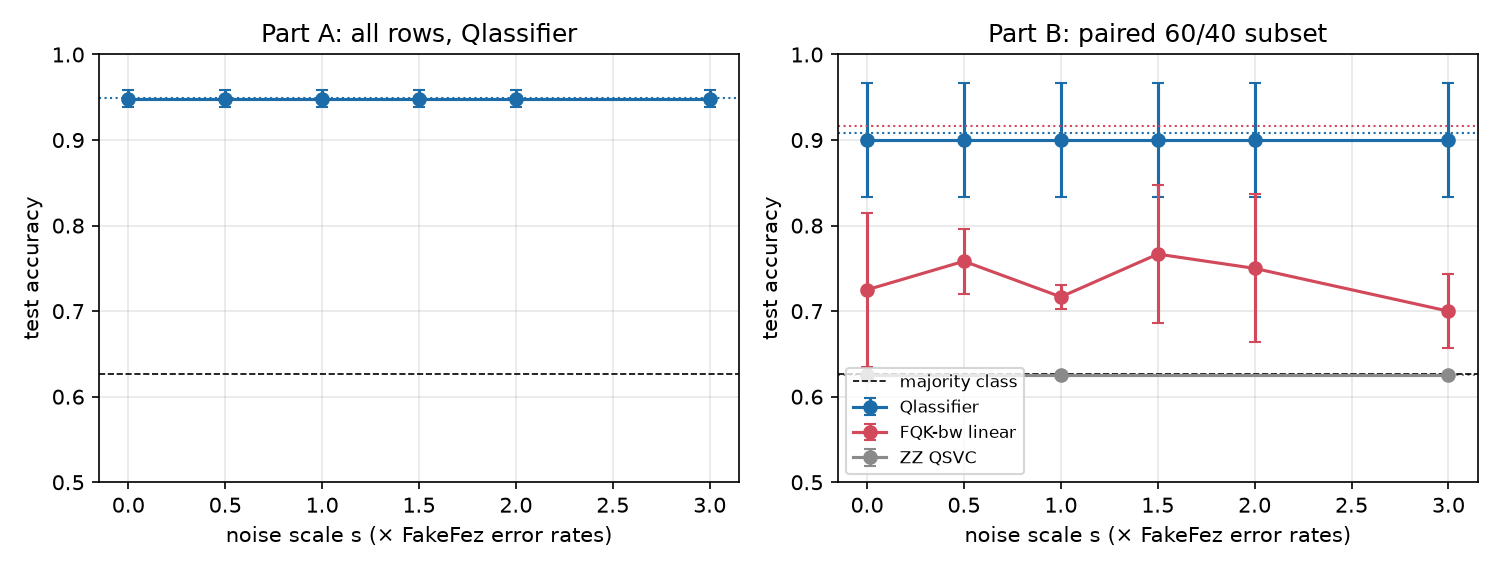
\includegraphics[width=\columnwidth]{breast_cancer-noise-sweep}
\caption{Accuracy vs noise scale $s$ (FakeFez error rates $\times s$), Breast Cancer paired subsets, \val{noise.shots}
shots. Dashed: exact simulation.}
\label{fig:sweep}
\end{figure}

\subsection{On a real quantum processor}
\label{sec:hardware}
On \val{hw.date} we ran Qlassifier on \val{hw.backend}, an IBM \val{hw.family} processor, through Qiskit Runtime (job
\code{\val{hw.jobid}}, \val{hw.time}). The task is the Part~B Breast Cancer subset of seed 0 (\val{hw.ntrain} training and
\val{hw.ntest} test rows). Training, tuning and the exact prediction used the simulator; the device measured the Bloch
readout of all \val{hw.ntrain} + \val{hw.ntest} rows: \val{hw.circuits} circuits (three Pauli settings per row) at
\val{hw.shots} shots, \val{hw.totalshots} shots in all. The circuits use \val{hw.qubits} physical qubits (\val{hw.layout}),
depth \val{hw.depth} and \val{hw.twoq} two-qubit gates after transpilation; Table~\ref{tab:hardware} gives their
calibration at submission. The job was billed \val{hw.qpu} QPU seconds (\val{hw.qpu.percircuit} s per circuit), inside
the \val{hw.qpu.low}--\val{hw.qpu.high} s predicted by our QPU cost model, which brackets the
published per-circuit timings of Table~\ref{tab:cost}'s sources as well.

Before submission we wrote down the FakeFez model's prediction for this exact subset: accuracy \val{hw.pred} $\pm$
\val{hw.pred.sd} over \val{hw.pred.draws} shot-noise draws (range \val{hw.pred.min}--\val{hw.pred.max}; exact simulation \val{hw.exact}),
and the pass rule, within 2\pp\ of the prediction. The hardware gave accuracy \val{hw.acc} (\val{hw.correct} of
\val{hw.ntest} rows; balanced accuracy \val{hw.ba}), \val{hw.delta}\pp\ above the prediction and at the top of its
shot-noise range. The measured kernel correlates with the exact one at $r = \val{hw.r}$ (training block
\val{hw.r.train}), and the mean Bloch-vector error is \val{hw.bloch} against \val{hw.bloch.pred} simulated. The result is
consistent with the prediction. We then ran \val{hw.all.later} more seeds of the same design
on the same device (Table~\ref{tab:hwseeds}); their predictions were computed by the same procedure after the runs,
so they are checks, not pre-registered tests. Over all \val{hw.all.seeds} seeds the hardware accuracy is
\val{hw.all.acc.min}--\val{hw.all.acc.max} (mean \val{hw.all.acc.mean}) against predictions of
\val{hw.all.pred.min}--\val{hw.all.pred.max} (mean \val{hw.all.pred.mean}); \val{hw.all.pass} of \val{hw.all.seeds}
seeds lie within 2\pp\ of their prediction and \val{hw.all.inrange} inside the shot-noise range; the mean deviation is
\val{hw.all.delta.mean}\pp\ (largest \val{hw.all.delta.absmax}\pp), the kernel correlation at least \val{hw.all.r.min},
and the whole study cost \val{hw.all.qpu} QPU seconds. The evidence is limited to a single device and calibration day, with
\val{hw.ntest} test rows per seed, so one row is \val{hw.rowpp}\pp\ and the pass rule is a one-row tolerance. The full
records (job ids, timestamps, transpiled circuits, raw counts, calibration before and after) are in the repository
(Sec.~\ref{sec:repro}).

\begin{table*}[t]
\centering
\caption{Every real-device run on \val{hw.backend}: the pre-registered seed 0 and the later seeds. Predicted = FakeFez
device model (mean $\pm$ sd over shot-noise draws); $\Delta$ = hardware $-$ predicted; kernel $r$ = correlation of the
measured test kernel with the exact one.}
\label{tab:hwseeds}
{\small% Generated by scripts/paper_tables.py from the saved results. Do not edit: rerun the script.
\begin{tabular}{rlrrrrrrr}
\hline
Seed & Job & QPU s & Exact & Predicted & Hardware & $\Delta$ (pp) & Within 2 pp & Kernel $r$ \\
\hline
0 & \code{dbesrqnpc3tc739mb92g} & 82 & 0.875 & 0.880 $\pm$ 0.010 & 0.900 & +2.0 & yes & 0.999 \\
1 & \code{dbeutp8m94ac738silb0} & 82 & 0.975 & 0.975 $\pm$ 0.000 & 0.975 & 0.0 & yes & 0.998 \\
2 & \code{dbeuv97pc3tc739mf740} & 82 & 0.875 & 0.874 $\pm$ 0.010 & 0.875 & +0.1 & yes & 0.999 \\
3 & \code{dbev0anpc3tc739mf97g} & 82 & 0.975 & 0.975 $\pm$ 0.000 & 0.975 & 0.0 & yes & 0.999 \\
4 & \code{dbev157sstms73fcr4s0} & 82 & 0.950 & 0.954 $\pm$ 0.009 & 0.950 & $-$0.4 & yes & 0.999 \\
\hline
\end{tabular}
}
\end{table*}

\begin{table}[t]
\centering
\caption{Physical qubits of the \val{hw.backend} run and their calibration at submission (\val{hw.date}).}
\label{tab:hardware}
{\small% Generated by scripts/paper_tables.py from the saved results. Do not edit: rerun the script.
\begin{tabular}{rrrrr}
\hline
Physical qubit & $T_1$ ($\mu$s) & $T_2$ ($\mu$s) & $\sqrt{X}$ error ($10^{-4}$) & Readout error (\%) \\
\hline
4 & 117 & 104 & 3.0 & 0.38 \\
2 & 148 & 128 & 1.4 & 0.45 \\
130 & 158 & 153 & 4.1 & 0.28 \\
50 & 108 & 94 & 4.1 & 0.23 \\
\hline
\end{tabular}
}
\end{table}

\subsection{Three more datasets}
\label{sec:stage2data}
We ran the same protocol (same splits, features, tuning budgets and \val{bc.seeds} seeds) on three more UCI
datasets (Table~\ref{tab:stage2}). On Spambase
(\val{s2.spambase.rows} rows) Qlassifier reaches BA \val{s2.spambase.q} against \val{s2.spambase.zz} for the ZZ baseline
(\val{s2.spambase.vszz}\pp, CI \val{s2.spambase.vszz.ci}, \val{s2.spambase.vszz.wins} seeds); on
Banknote \val{s2.banknote.q} against \val{s2.banknote.zz} (\val{s2.banknote.vszz}\pp). Both tie the best classical model (\val{s2.spambase.vsbest}\pp\ vs \val{s2.spambase.best}, CI
\val{s2.spambase.vsbest.ci}; \val{s2.banknote.vsbest}\pp\ vs \val{s2.banknote.best}), but on Spambase the MLP is ahead
of Qlassifier by a small, significant margin (\val{s2.spambase.vsmlp}\pp, CI \val{s2.spambase.vsmlp.ci}): a tie with the
best model does not mean a tie with every model. On Haberman (\val{s2.haberman.rows} rows) every model lands between
\val{s2.haberman.q} and \val{s2.haberman.best.ba}, and every pair of models
ties. The ZZ margin is dataset-specific: \val{s2.spambase.vszz} and \val{s2.banknote.vszz}\pp\ here
against \val{uci.vszz.min} to \val{uci.vszz.max}\pp\ on the first four datasets. These datasets are not bundled in the
released library yet; the results come from the research scripts in the repository.

\begin{table*}[t]
\centering
\caption{Three more UCI datasets under the same protocol (balanced accuracy, mean $\pm$ sd over \val{bc.seeds} seeds;
corrected CIs).}
\label{tab:stage2}
{\small% Generated by scripts/paper_tables.py from the saved results. Do not edit: rerun the script.
\begin{tabular}{lrrrrr}
\hline
Dataset & Rows & Qlassifier BA & ZZ QSVC BA & $\Delta$ vs ZZ [CI] (wins) & $\Delta$ vs best classical [CI] \\
\hline
Spambase & 4,601 & 0.911 $\pm$ 0.006 & 0.899 & +1.2 [+0.8, +1.6] (10/10) & $-$0.8 [$-$2.0, +0.4] vs Gradient boosting \\
Banknote & 1,372 & 1.000 $\pm$ 0.001 & 0.955 & +4.4 [+2.7, +6.2] (10/10) & 0.0 [$-$0.2, +0.2] vs MLP \\
Haberman & 306 & 0.564 $\pm$ 0.031 & 0.546 & +1.9 [$-$4.1, +7.9] (6/10) & $-$1.8 [$-$8.1, +4.4] vs MLP \\
\hline
\end{tabular}
}
\end{table*}

\subsection{Cost and time}
On Breast Cancer, Qlassifier needs \val{bc.circuits} circuits to train and predict. The bandwidth-tuned fidelity-kernel
pipeline needs \val{bc.circuits.fqkpipeline}, mostly for its on-device bandwidth search: \val{bc.circuitratio} times
more (BT-7; Table~\ref{tab:cost}, Fig.~\ref{fig:cost}). Counting only its final Gram matrices, without the search,
the pipeline needs \val{bc.circuits.fqkfinal} circuits, \val{bc.circuitratio.final} times Qlassifier's; both readings
hold. The projected kernel matches Qlassifier's circuit count but needs two-qubit gates. The full Breast Cancer leaderboard (\val{bc.seeds} seeds, \val{bc.models} models) runs in \val{bt10.wall}\,s
on an \val{bt10.cpu} laptop with \val{bt10.cores} cores (BT-10). There, tuning Qlassifier over its
\val{protocol.configs} configurations takes a median of \val{bc.time.tune}\,s per split, and the final fit
\val{bc.time.fit}\,s.

\begin{table*}[t]
\centering
\caption{Breast Cancer cost study: qubits, two-qubit gates and depth per circuit after transpilation to IBM FakeTorino,
FakeFez and FakeBrisbane, and circuits to train and predict ($N_\text{train} = \val{bc.ntrain}$,
$N_\text{test} = \val{bc.ntest}$). Fidelity kernels need one circuit per pair of rows; models whose hyperparameters
change the circuit also pay for the on-device search.}
\label{tab:cost}
{\small% Generated by scripts/paper_tables.py from the saved results. Do not edit: rerun the script.
\begin{tabular}{lrcrrrr}
\toprule
 & & 2Q gates & Depth & \multicolumn{3}{c}{Circuits} \\
Model & Qubits & Torino / Fez / Brisbane & Torino & train + predict & tuning on device & total \\
\midrule
PQK & 9 & 72 / 72 / 72 & 165 & 1,707 & 0 & 1,707 \\
\textbf{Qlassifier} & 4 & 0 / 0 / 0 & 6 & 1,707 & 0 & 1,707 \\
ZZ QSVC & 8 & 393 / 428 / 394 & 623 & 147,061 & 0 & 147,061 \\
FQK-bw full & 8 & 393 / 428 / 394 & 623 & 147,061 & 2,276,238 & 2,423,299 \\
FQK-bw linear & 8 & 54 / 54 / 54 & 133 & 147,061 & 2,276,238 & 2,423,299 \\
Separable & 8 & 0 / 0 / 0 & 6 & 147,061 & 2,276,238 & 2,423,299 \\
\bottomrule
\end{tabular}
}
\end{table*}

\begin{figure*}[t]
\centering
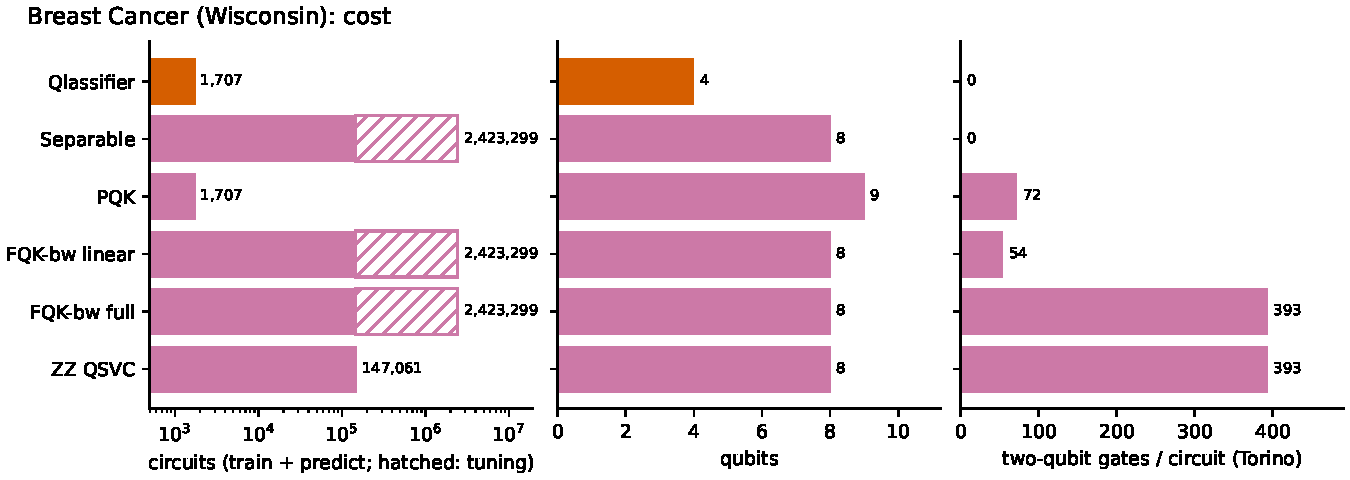
\includegraphics[width=0.9\textwidth]{breast_cancer-cost}
\caption{Breast Cancer cost per quantum model: circuits to train and predict (log scale; hatched: on-device tuning),
qubits, and two-qubit gates per circuit on FakeTorino.}
\label{fig:cost}
\end{figure*}

\subsection{Targets}
Table~\ref{tab:targets} lists the ten targets as the library evaluates them: \val{targets.met} are met and
\val{targets.reportonly} is report-only (\val{targets.reportonly.ids}). BT-6 (beat every tuned classical model with a
CI above zero) is report-only: it was missed under the strict protocol before this run (Table~\ref{tab:history}), and
by our pre-registered rule no later run can upgrade it. BT-8 is met on the core datasets (qubits
$\leq \lceil d/2 \rceil$, no two-qubit gates) and on the protein angles, where geometry mode uses \val{protein.qubits}
qubits for \val{protein.features} angles: the $\lceil d/2 \rceil$ bound applies to the core encoding, and geometry mode
is judged by one qubit per circle or direction (Sec.~\ref{sec:limits}).

\begin{table*}[t]
\centering
\caption{Benchmark targets BT-1 to BT-10 as evaluated by \code{qlassifier benchmark} (\code{targets.json}).}
\label{tab:targets}
{\small% Generated by scripts/paper_tables.py from the saved results. Do not edit: rerun the script.
\begin{tabular}{lp{0.36\textwidth}p{0.38\textwidth}l}
\toprule
Target & Pass rule & Measured & Status \\
\midrule
BT-1 & Breast Cancer: mean accuracy Qlassifier $-$ ZZ QSVC $\geq$ 20 pp & 0.956 vs 0.677 $\rightarrow$ +27.9 pp & met \\
BT-2 & mean BA Qlassifier $>$ ZZ QSVC on all 5 datasets; paired win rate $\geq$ 0.8 on each & breast\_cancer +37.6 pp (10/10); ionosphere +22.6 pp (10/10); sonar +27.9 pp (10/10); heart +28.3 pp (10/10); protein\_angles +35.5 pp (10/10) & met \\
BT-3 & mean BA $\geq$ published $-$ 1 pp on $\geq$ 3 of 4 UCI sets (0.968 / 0.911 / 0.813 / 0.804) & breast\_cancer 0.948 ($-$2.0 pp); ionosphere 0.925 (+1.4 pp); sonar 0.824 (+1.1 pp); heart 0.816 (+1.2 pp) $\rightarrow$ 3/4 & met \\
BT-4 & mean BA $\geq$ published on $\geq$ 2 of 4 UCI sets & breast\_cancer 0.948 ($-$2.0 pp); ionosphere 0.925 (+1.4 pp); sonar 0.824 (+1.1 pp); heart 0.816 (+1.2 pp) $\rightarrow$ 3/4 & met \\
BT-5 & mean BA over the 4 UCI sets: Qlassifier highest among the in-harness quantum models & qlassifier 0.878, separable 0.870, fqk\_bandwidth\_full 0.864, pqk 0.862, fqk\_bandwidth\_linear 0.856, zz\_qsvc 0.587 & met \\
BT-6 & $\geq$ 1 dataset: mean BA above every tuned classical model and corrected 95\% CI of $\Delta$ vs best classical $>$ 0 (stretch; report-only) & breast\_cancer vs mlp: $-$1.3 [$-$3.1, +0.5] pp (tie); ionosphere vs rbf\_svm: $-$0.2 [$-$3.1, +2.7] pp (tie); sonar vs mlp: +0.5 [$-$8.5, +9.5] pp (tie); heart vs logistic\_regression: $-$1.0 [$-$3.1, +1.2] pp (tie); protein\_angles vs gradient\_boosting: +1.0 [$-$0.2, +2.2] pp (tie) & report-only \\
BT-7 & Breast Cancer: $\geq$ 100$\times$ fewer circuits than the bandwidth-tuned fidelity-kernel pipeline (incl. its search) & 1,707 vs 2,423,299 $\rightarrow$ 1,420$\times$ & met \\
BT-8 & per circuit on FakeTorino / FakeFez / FakeBrisbane: core encoding qubits $\leq$ ceil(d/2); geometry mode: 1 qubit per circle or (lat, lon) pair + ceil(d\_plain/2); 2Q gates $\leq$ n $-$ 1 & breast\_cancer: 4 qubits (core, ceil(8/2) = 4), 0 two-qubit gates; ionosphere: 4 qubits (core, ceil(8/2) = 4), 0 two-qubit gates; sonar: 4 qubits (core, ceil(8/2) = 4), 0 two-qubit gates; heart: 4 qubits (core, ceil(8/2) = 4), 0 two-qubit gates; protein\_angles: 10 qubits (geometry limit 10), 0 two-qubit gates & met \\
BT-9 & Breast Cancer, 1,024 shots: mean accuracy drop $\leq$ 2 pp on each device (part A); $<$ FQK-bw drop (part B) & part A drop 0.12 / 0.12 / 0.12 pp (Torino / Fez / Brisbane); part B Qlassifier 0.8 / 0.8 / 0.8 vs FQK-bw linear 22.5 / 20.0 / 17.5 pp & met \\
BT-10 & \texttt{qlassifier benchmark breast\_cancer}, defaults, exact, Apple M-class laptop: wall $\leq$ 120 s & 56.2 s on Apple M4 (10 cores, macOS-27.0-arm64-arm-64bit; 1-min load 1.95 at start) & met \\
\bottomrule
\end{tabular}
}
\end{table*}

% ---------------------------------------------------------------------------------------------------------------------
\section{Related work and novelty}
\label{sec:related}

\textit{Known parts.} Dense angle encoding~\cite{larose2020robust} and trigonometric product feature
maps~\cite{stoudenmire2016supervised}; projected quantum kernels~\cite{huang2020power}; product and separable kernels as
strong baselines~\cite{bowles2024better,shin2025new}; the role of the bandwidth~\cite{shaydulin2021importance,%
canatar2022bandwidth,egginger2023a,florezablan2025on}; the Fourier view of angle
encodings~\cite{schuld2020the,repetto2026expressivity}; symmetry-aware and geometric
models~\cite{glick2021covariant,meyer2022exploiting,ragone2022representation,li2024enforcing}; stereographic Bloch
embeddings~\cite{jasso2023quantum}; directional statistics and torus methods for dihedral
angles~\cite{sra2016directional,pewsey2020recent,eltzner2015torus,wiechers2021clustering}; noise rescaling of quantum
kernels~\cite{haug2021quantum,hubregtsen2021training} and Pauli decompositions of fidelity kernels~\cite{gan2023a}; and
structure-aware encodings that beat tuned RBF on
synthetic or simulated data~\cite{wang2026structured,frohnert2026taskaligned}.

\textit{What is new here.} (i) The design rule: circuit angles fixed by the data scale or by the declared geometry,
bandwidth and margin tuned only after measurement. It costs zero tuning circuits and keeps the device noise loss small.
(ii) Geometry mode: one qubit per circle or direction, no aliasing, with the exact classical twin
reported next to it. (iii) The hardware protocol: three local-Pauli settings per sample ($O(N)$ circuits) with
per-qubit unit renormalisation. (iv) A benchmark of all of this against every challenge baseline on real data, with
leakage-safe splits, corrected statistics and the negative results kept (Sec.~\ref{sec:limits}). We found no prior
applied QML on protein dihedral angles with angle-native encodings.

% ---------------------------------------------------------------------------------------------------------------------
\section{Limitations}
\label{sec:limits}

\begin{itemize}
\item \textit{No quantum advantage.} Qlassifier prepares product states, which a classical computer simulates exactly;
  the library's default mode does just that. In geometry mode the classical twin reproduces the kernel by construction.
  Our results are measured gains over quantum baselines and ties with classical ones.
\item \textit{BT-6 missed.} We did not beat every tuned classical model on any dataset under a leakage-safe protocol.
  A residue-level split showed \val{e07.vsbest}\pp\ (CI \val{e07.vsbest.ci}) over \val{e07.best}, but it shares
  protein chains between training and test. Under chain-grouped splits the margin shrank to \val{e11.vsbest}\pp\ (CI
  \val{e11.vsbest.ci}), and two pre-registered tests on \val{protein.chains} chains gave \val{e12.div6.vsbest}\pp\ (\val{e12.div6.level}\% CI
  \val{e12.div6.vsbest.ci}) and \val{e12.div10.vsbest}\pp\ (\val{e12.div10.level}\% CI \val{e12.div10.vsbest.ci}).
\item \textit{A loss: global earthquakes.} On \val{quakes.rows} earthquakes labelled by depth from their latitude and
  longitude (USGS), geometry mode lost to \val{quakes.best} by \val{quakes.vsbest}\pp\ (CI \val{quakes.vsbest.ci}),
  although it beat RBF-SVM by \val{quakes.vsrbf}\pp. A wider kernel grid closed part of the gap
  (\val{quakes.wide.vsrf}\pp, CI \val{quakes.wide.vsrf.ci}). Trees adapt to the uneven density of subduction zones;
  one global kernel width does not. The narrow kernels this task needs also need far more than \val{noise.shots} shots.
\item \textit{Limited hardware evidence.} Beyond the device models we have \val{hw.all.seeds} real runs
  (Sec.~\ref{sec:hardware}) on one device under one day's calibration, \val{hw.ntest} test rows each; only the first
  was pre-registered. The device models have no crosstalk, drift or leakage,
  no idle noise and symmetric readout errors; the per-qubit simulation is exact only under these assumptions. At
  \val{noise.shots} shots the simulated study cannot rank the three devices (Sec.~\ref{sec:results}).
\item \textit{The fidelity kernel's loss is mostly shot noise.} Its \val{bc.noiseb.fqk.min}--\val{bc.noiseb.fqk.max}\pp\
  loss under device models is \val{sweep.fqk.drop0}\pp\ with device noise off (Sec.~\ref{sec:sweep}); Qlassifier's advantage
  over it comes from shot efficiency: three settings per sample instead of one fidelity per pair.
\item \textit{The ZZ margin varies.} On Spambase and Banknote the lead over the ZZ baseline is \val{s2.spambase.vszz}
  and \val{s2.banknote.vszz}\pp, not tens of points, and on Haberman every model ties (Sec.~\ref{sec:stage2data}).
\item \textit{Not in the library yet.} The hardware run, the noise sweep and the three extra datasets are research
  results with scripts in the repository; the released library has no hardware backend or noise-sweep API (it does
  benchmark a user's CSV file under the same protocol). They are planned for a later release.
\item \textit{More qubits in geometry mode.} Geometry mode uses one qubit per circle, above the $\lceil d/2 \rceil$
  of the core encoding (\val{protein.qubits} qubits for the \val{protein.features} protein angles), because two
  circles cannot share a qubit (Sec.~\ref{sec:geometry}). The hardware target counts geometry mode by this rule;
  the circuits stay free of two-qubit gates, so the device cost per circuit is unchanged.
\item \textit{Small data, wide intervals.} The UCI test sets hold \val{uci.ntest.min} to \val{uci.ntest.max} rows. With \val{bc.seeds} seeds, the
  corrected CIs are wide.
\item \textit{Scope.} Binary classification of tabular data with up to \val{limit.trainrows} training rows (the Gram
  matrix is $N \times N$).
\end{itemize}

% ---------------------------------------------------------------------------------------------------------------------
\section{Reproducibility}
\label{sec:repro}

Install the library from the repository (\repo) with \code{pip install .} (Python 3.12), then run
\begin{center}
\code{qlassifier benchmark --noise}
\end{center}
to reproduce every leaderboard, noise and cost number of this paper. The saved results come from two runs on one
\val{run.cpu} laptop (\val{run.cores} cores): the UCI datasets with \val{run.uci.jobs} workers (about
\val{run.uci.min}\,min, commit \val{run.uci.commit}) and the protein angles with \val{run.protein.jobs} workers (about
\val{run.protein.min}\,min, commit \val{run.protein.commit}), because ten parallel \val{protein.qubits}-qubit noise cells exhausted the
laptop's memory. The worker count changes wall time only: every task is seeded by dataset, seed and model, and the two
versions produce bit-identical device samples (\path{benchmarks/README.md}). Before the run, the engine reproduced
\val{golden.rows} of \val{golden.rows} rows of the method search's reference leaderboard with \val{golden.mismatches}
mismatches (chosen configuration and every metric within $10^{-9}$; \path{benchmarks/golden_e01.txt}). Across
platforms, BLAS rounding can move a ROC-AUC by one resolution step and the MLP by more. Every result file
records the versions (Qlassifier \val{version.qlassifier}, Qiskit \val{version.qiskit}, Qiskit Aer
\val{version.qiskitaer}, scikit-learn \val{version.scikitlearn}, NumPy \val{version.numpy}) and the protocol fingerprint
(\code{\val{protocol.fingerprint}}). Results depend only on dataset, seed, model and versions, not on scheduling. The
saved results, per-seed tables and plots are in \path{benchmarks/}. The script
\path{scripts/paper_tables.py} writes every number of this paper from them, and the CI fails when they drift apart. The
method-search experiments behind Table~\ref{tab:history} are in \path{experiments/classifier/}. The
results (Secs.~\ref{sec:sweep}, \ref{sec:hardware}, \ref{sec:stage2data}) are in
\path{experiments/hardware/} with their scripts and raw outputs; the hardware record is
\path{e07-hardware-point/run-seed0/record.json}, and the same script reproduces the numbers of those sections. The command
\code{qlassifier ui} opens a local dashboard with the same leaderboards, noise and cost views.

% ---------------------------------------------------------------------------------------------------------------------
\section{Conclusion}
\label{sec:conclusion}

A quantum kernel classifier can be good by default and cheap on hardware if it keeps its circuits fixed and tunes
after the measurement. Against the standard ZZ baseline, Qlassifier gains \val{uci.vszz.min} to \val{uci.vszz.max}\pp\ BA on the UCI
datasets; it ties tuned classical models, has the highest mean BA of the quantum models in our harness, and loses at
most \val{noise.max}\pp\ under IBM device noise models, with few qubits and no two-qubit gates. \val{hw.all.seeds} runs on an IBM Heron processor returned the accuracy the device model predicted,
for \val{hw.all.qpu} QPU seconds in all. Where the data has geometry, geometry mode encodes it directly, but the gain comes from the geometric
prior, as the classical twin shows. The benchmark, including its ties and losses, ships with the library for reuse.

\bibliography{refs}

\end{document}
